\documentclass[10pt,a4paper,oneside]{scrbook}
\usepackage[utf8]{inputenc}     % Set UTF-8 input encoding
\usepackage[italian]{babel}     % Set up italian language
\usepackage{amsmath}            % Additional things
\usepackage{amsfonts}           % Additional things
\usepackage{amssymb}            % Additional symbols
\usepackage[dvipsnames]{xcolor} % Load colors
\usepackage{graphicx}           % Load graphics in document
\usepackage{frontespizio}       % For the first page
\usepackage{microtype}          % Additional symbols
\usepackage{textcomp}           % Additional symbols
\usepackage{hyperref}           % For links
\usepackage{tikz}               % Load TiKZ
\usepackage{pgfplots}           % Load graph tools
\usepackage{enumitem}           % For changing item bullets
\usepackage{minted}             % For source code listing
\usepackage{tcolorbox}          % For source code frames

% Make clickable links in document
\hypersetup{
    colorlinks,
    citecolor=black,
    filecolor=black,
    linkcolor=black,
    urlcolor=black
}

% TiKZ settings
\usetikzlibrary{tikzmark}
\usetikzlibrary{calc}
\usetikzlibrary{shapes,snakes}

% Create useful environments for source code listing
\tcbuselibrary{skins,minted}
\newtcblisting{sourcecode}[1]{ % Generic source code environment, the argument is the language
    boxrule=1pt,
    listing only,
    listing engine=minted,
    minted language=#1,
    minted options={tabsize=2,escapeinside=??}
}
\newtcblisting{systemc}[1]{ % SystemC source code environment, the argument is the file title
    enhanced,
    title={#1\strut}, 
    fonttitle=\bfseries, 
    attach boxed title to top left={xshift=3.2mm,yshift=-0.50mm}, 
    boxed title style={skin=enhancedfirst jigsaw,size=small,arc=1mm,bottom=-1mm}, 
    listing only,
    minted language=cpp,
    minted options={tabsize=2,escapeinside=??}
}
\newtcblisting{vhdl}[1]{ % VHDL source code environment, the argument is the 
%file title
    enhanced,
    title={#1\strut}, 
    fonttitle=\bfseries, 
    attach boxed title to top left={xshift=3.2mm,yshift=-0.50mm}, 
    boxed title style={skin=enhancedfirst 
    jigsaw,size=small,arc=1mm,bottom=-1mm}, 
    listing only,
    minted language=vhdl,
    minted options={tabsize=2,escapeinside=??}
}

\begin{document}
\begin{frontespizio}
    \Universita{Verona}
    \Dipartimento{Informatica}
    \Corso{Ingegneria Informatica}
    \Annoaccademico{2018--2019}
    \NCandidati{Autori}
    \Candidato{Matteo Iervasi}
    \Candidato{Linda Sacchetto}
    \Candidato{Leonardo Testolin}
    \Titolo{Appunti di Progettazione di Sistemi Embedded}
\end{frontespizio}

\tableofcontents
\newpage

\chapter*{Prefazione}
Questa dispensa si basa sugli appunti di Linda Sacchetto e Leonardo Testolin durante il
corso di \textit{Progettazione di Sistemi Embedded} dell'anno accademico 2018/2019.
Nonostante sia stata revisionata in corso di scrittura, potrebbe contenere errori di vario tipo.
In tal caso potete segnalarli inviando una mail all'indirizzo \href{mailto:matteoiervasi@gmail.com}{matteoiervasi@gmail.com}.

\hspace*{\fill} Matteo Iervasi

\chapter{Introduzione}
Citando Wikipedia, un sistema embedded, nell'informatica e nell'elettronica,
identifica genericamente tutti quei sistemi elettronici di elaborazione digitale a microprocessore progettati
appositamente per una determinata applicazione (special purpose), ovvero non riprogrammabili dall'utente per altri scopi,
spesso con una piattaforma hardware ad hoc, integrati nel sistema che controllano ed in grado di gestirne tutte o
parte delle funzionalità richieste.

Storicamente, sono nati prima i sistemi embedded rispetto ai sistemi \textit{general purpose}, basti pensare ai
grandi calcolatori degli anni '40. Essi infatti erano costruiti per un utilizzo specifico, anche se in quanto a 
dimensioni non erano di certo ristretti.
Tuttavia il primo vero sistema embedded, in tutti i sensi, fu l'\textit{Apollo Guidance Computer}, che doveva
contenere una notevole potenza computazionale per il tempo in spazi ristrettissimi. La produzione di massa di 
sistemi embedded cominciò con l'\textit{Autonetics~D-17} nel 1961 e continua fino ai nostri giorni.

Non possiamo progettare i sistemi embedded come facciamo con i sistemi \textit{general purpose}, perché abbiamo
dei vincoli di progettazione e degli obiettivi differenti. Se ad esempio nei sistemi \textit{general purpose} la
ricerca si focalizza nel costruire processori sempre più veloci, nei sistemi embedded la CPU esiste solamente come
un modo per implementare algoritmi di controllo che comunica con sensori ed attuatori, e diventa invece più 
interessante trovare processori che usano sempre meno energia.

I vincoli principali ai quali bisogna attenersi durante la progettazione di un sistema embedded sono:
\begin{itemize}
    \item \textbf{Dimensione e peso}\\
          Si pensi ai dispositivi che devono poter essere tenuti in una mano
    \item \textbf{Energia}\\
          Molto spesso i dispositivi embedded devono funzionare con una batteria
    \item \textbf{Ambiente esterno ostile}\\
          Bisogna dover tenere conto di eventuali fluttuazioni di energia, interferenze radio, calore, acqua, ecc.
    \item \textbf{Sicurezza e operazioni \textit{real time}}\\
          Vi sono casi in cui è necessario che il sistema debba garantire sempre il funzionamento, oppure che 
          garantisca un tempo costante per ogni operazione
    \item \textbf{Costi contenuti}\\
          Oltre a tutto il resto, bisogna tenere i costi bassi altrimenti si rischia di non poter vendere il prodotto
\end{itemize}

\chapter{Modellazione dei sistemi embedded}
Nel momento in cui ci accingiamo a pensare a come si progetta un sistema embedded, salta subito alla mente un
problema, ovvero come faccio a verificarne il corretto funzionamento?
Quando progettiamo del software, abbiamo a disposizione una miriade di strumenti per assicurarci di tenere il numero
dei bug il più basso possibile: \textit{debugger}, \textit{unit testing}, \textit{analisi statica}, ecc.
In hardware invece non possiamo certamente metterci a rifare tutto ogni volta che sbagliamo, ricordiamoci che dobbiamo
tenere i costi bassi! Si pone quindi il problema della \textit{simulazione}, strumento fondamentale per la verifica
del nostro sistema. Spesso infatti l'architettura di riferimento è differente da quella del calcolatore che usiamo
per lo sviluppo (caso tipico: noi sviluppiamo su architettura X86 per un'architettura di destinazione ARM).

\smallskip
In generale, un sistema embedded è costituito dalle seguenti componenti:
\begin{itemize}
	\item \textbf{Piattaforma hardware}\\
    Oltre al microprocessore, vi sono una serie di altre componenti.
	\item \textbf{Componenti software}\\
    Il software è monolitico: quando accendo il sistema, si esegue in automatico.
    Possono anche esserci casi in cui è necessario caricare un intero sistema operativo, e nella maggioranza di essi si fa riferimento a Linux.
	\item \textbf{Componenti analogiche} (es. sensori e trasduttori)\\
    Naturalmente se il nostro sistema dovrà interagire con l'ambiente esterno dovremmo introdurre componenti analogiche.
\end{itemize}
Il trend attuale è di portare tutto ciò in un singolo chip (SoC - \textit{System on a Chip}), dove microprocessore,
memoria e altre componenti vengono montate su un singolo chip, collegate da un bus. Esempi di SoC moderni sono i
Qualcomm\textsuperscript{\textregistered} Snapdragon o i Samsung\textsuperscript{\textregistered} Exynos.
Esiste anche un'alternativa, dove le componenti invece di trovarsi in un unico chip si trovano in una singola
board (SoB - \textit{System on a Board}).

Queste due tecnologie hanno uno scopo in comune: indurre al riutilizzo di componenti già esistenti per
ridurre il più possibile il \textit{time to market} (figura \ref{img:time-to-market}), ovvero il tempo che trascorre
dall'inizio della progettazione all'immissione nel mercato. Più questo tempo è lungo, meno probabilità si ha di riuscire a vendere
il prodotto in quantità tale da coprire i costi di sviluppo.
Per questo motivo non si può minimamente pensare di sviluppare un sistema embedded partendo da zero, in quanto il tempo di sviluppo
sarebbe improponibile.

\begin{figure}
	\centering
	\caption{Rappresentazione del rapporto costo produzione - guadagno}
	\label{img:time-to-market}
	\begin{tikzpicture}
		\centering
		\begin{axis}[
			axis lines=left,
			width=\textwidth,
			height=200pt,
            xmin=0,
			xlabel=Tempo,
			ylabel=Costo,
            yticklabels={,,},
            xticklabels={,,},
		]
		\addplot[
			domain=0:7,
			samples=150,
			color=blue,
			line width=1.25pt,
		]{5*ln(x-1/2)+3};
        \addlegendentry{Costo di produzione}
        \addplot[
            domain=1.25:7,
   			samples=150,
   			color=red,
   			line width=1.25pt,
        ]{20/ln(x)-20};
        \addlegendentry{Prezzo di vendita}
		\end{axis}
        \draw [dashed] (0.9,0) node [below]{$t_0$};
        \draw [dashed] (2,0) node [below]{$t_m$} -- (2,5.5);
        \draw [dashed] (3.6,0) -- (3.6,1.4);
        \draw [<->](2,0.70) -- (3.6,0.70) node [below, midway] {$\Delta_t$};
        \draw [->] (0.9,-0.45) -- (1,-1) node [below] {Inizio realizzazione oggetto};
        \draw [->] (2,-0.45) -- (4,-1.5) node [below] {Inizio vendita oggetto};
	\end{tikzpicture}
\end{figure}

\section{Co-design di sistemi embedded}
Viste le ristrettezze imposte sui tempi dal mercato, è necessario ricorrere al co-design di hardware e software.
Si parte quindi con una descrizione generale del sistema, magari aiutandosi con un prototipo, dopodiché fatte le verifiche su di esso si procede con la separazione di
hardware e software, ricordandosi che è necessario ‘‘riciclare’’ il più possibile le parti già esistenti, si comincia lo sviluppo o l'eventuale adattamento.
Durante la progettazione della parte hardware, si può decidere di affiancare l'eventuale processore da un co-processore, che svolge un compito
specifico a seconda di cosa stiamo progettando. Il co-processore può essere anche una GPU.

Le tecnologie più usate per la progettazione di hardware sono:
\begin{itemize}
	\item Microcontrollore standard o microprocessore
	\item ASIC (con o senza co-processore a seconda dei casi)
	\item FPGA
\end{itemize}
mentre per il software si possono utilizzare diversi linguaggi di programmazione (generalmente però si scelgono C/C++).

Naturalmente ci serve uno strumento per la verifica del nostro sistema, ci serve quindi co-simulare hardware e software.
Si può fare su diversi livelli, ognuno con i suoi pregi e i suoi difetti.
\begin{itemize}
	\item \textbf{Gate level}\\
	Viene simulato il tutto a livello di porte logiche, ovvero il più basso livello
	possibile. Questa è la simulazione più lenta in assoluto.
	\item \textbf{RTL (Register Transfer Level)}
	La rappresentazione in questo caso è vista come un flusso di informazioni che
	percorre il sistema, i cui risultati vengono salvati nei registri. Anche questa
	simulazione è lenta poiché molto vicina all'hardware.
	Essa può essere \textit{cycle accurate}, nella quale l'unità minima di elaborazione è il ciclo
	di clock dove è considerato come importante quello che avviene all'inizio e alla fine di esso,
	oppure può essere \textit{instruction accurate}, nella quale l'unità minima diventa la singola istruzione.
	\item \textbf{Behavioural}\\
	Questa rappresentazione descrive le funzionalità facendo una stima dei cicli di clock che impiega
	\item \textbf{Transactional}\\
	In questo caso non ho nemmeno il dettaglio della funzionalità, ma vado solamente a descrivere
	le interazioni tra i singoli moduli hardware. La simulazione in questa modalità è rapida.
\end{itemize}

Ogni livello di descrizione ha dei linguaggi più adatti di altri nonostante siano stati fatti diversi
sforzi di crearne uno adatto a tutti.
A livello RT, quelli più diffusi sono \textit{VHDL} e \textit{Verilog}.
\textit{SystemC}, nonostante sia in grado di scrivere più o meno bene a livello RT, mostra la sua
potenza espressiva agli altri livelli.

\section{Hardware description languages}
Gli \textit{Hardware Description Languages} (HDL) sono nati per risolvere una serie di problemi.
Prima di essi l'hardware veniva progettato a mano e senza alcuna procedura standardizzata. Questo
approccio però è prono ad errori e soprattutto incompatibile con le tempistiche richieste al giorno d'oggi.
Quando progetto del software mi basta pensare all'algoritmo astratto e codificarlo in un preciso linguaggio
di programmazione. Può anche succedere che il linguaggio che utilizzo sia multipiattaforma, per cui non mi dovrò
minimamente preoccupare di dove e come verrà eseguito, poiché so che a prescindere dall'architettura sul quale
verrà eseguito darà sempre lo stesso risultato.
Quando progettiamo hardware invece non possiamo permetterci questo lusso in quanto l'architettura semplicemente
non c'è, siamo noi a costruirla.

Prendiamo in esempio un programma scritto in linguaggio C e osserviamo le assunzioni che facciamo senza nemmeno pensare.\\
\begin{sourcecode}{c}
#include <stdio.h>

int gcd(int xi, int yi){
   	int x, y, temp;
   	
   	x = xi;
   	y = yi;
   	while(x > 0){
   		if(x <= y){
   			temp = y;
   			y = x;
   			x = temp;
   		}
   		x = x - y;
   	}
   	return(y);
}

int main(int argc, char *argv[]){
   	int xi, yi, ou;
    
    scanf("%d %d", &xi, &yi);
    ou = gcd(xi, yi);
    printf("%d\n", ou);
    
    return 0;
}
\end{sourcecode}
I requisiti hardware per poter eseguire questo programma sono:
\begin{itemize}
    \item \textbf{Input/Output}\\
    \textit{SW}: \texttt{printf}, \texttt{scanf}, ...\\
    \textit{HW}: interfacce di I/O
    \item \textbf{Temporizzazione}\\
    \textit{SW}: istruzioni vengono eseguite alla velocità del ciclo di clock\\
    \textit{HW}: devono essere definiti uno o più segnali di clock (e le istruzioni possono impiegare diversi cicli di clock)
    \item \textbf{Dimensioni variabili}\\
    \textit{SW}: dimensioni implicite sono nascoste\\
    \textit{HW}: devo tenere conto delle dimensioni, in quanto sto creando qualcosa di fisico che poi corrisponderà alla variabile
    \item \textbf{Operazioni}\\
    \textit{SW}: esistono librerie per ogni tipo di operazioni\\
    \textit{HW}: difficili dato che devo fare un circuito apposito. Se poi vogliamo anche i numeri in virgola mobile, il circuito aumenta molto in complessità
    \item \textbf{Identificazione elementi di memoria}\\
    \textit{SW}: non guardo se una variabile va nei registri o nella RAM, la uso e basta\\
    \textit{HW}: devo sapere che spazio andrà a occupare, c'è una bella differenza tra registro e memoria
    \item \textbf{Sincronizzazione moduli}\\
    \textit{SW}: spesso lavoro in maniera sequenziale\\
    \textit{HW}: per com'è strutturato, l'hardware lavora tantissimo in parallelo        
\end{itemize}
Quando scriviamo l'algoritmo software facciamo quindi molte assunzioni, del tutto legittime, ma che non possiamo di certo dare per 
scontato quando invece progettiamo un modulo hardware.

\noindent
La prima cosa di cui bisogna preoccuparsi è definire le porte d'ingresso e di uscita. Una volta completata
l'identificazione delle porte, bisogna individuare la modalità con cui andremo a progettare il modulo,
che nel nostro caso sarà una FSMD, ovvero una macchina a stati finiti combinata con un datapath. 
Nella definizione della FSM e del DP, bisogna tenere conto degli eventuali vincoli: se ad esempio mi interessa un circuito veloce posso permettermi un DP più grande, mentre se voglio che il mio circuito occupi il minor spazio possibile dovrò allargare la FSM.
Riportiamo di seguito un possibile diagramma del modulo \texttt{gcd}.
\begin{figure}[h]
    \centering
    \begin{tikzpicture}
        \draw [->] (0,2) node[above]{XI} -- (1,2);
        \draw [->] (0,1) node[above]{YI} -- (1,1);
        \draw [<-] (2,3) -- (2,4) node[left]{CLOCK};
        \draw [<-] (4,3) -- (4,4) node[left]{RESET};
    
        \draw [fill=SkyBlue] (1,0) rectangle (5,3) node[pos=.5] {GCD};
        
        \draw [->] (5,1.5) -- (6,1.5) node [above] {OUT};
    \end{tikzpicture}
    \label{img:gcd_scheme}
    \caption{Schema di un modulo GCD}
\end{figure}

\pagebreak\noindent
Questa è una possibile implementazione in VHDL del modulo GCD, descritta dal punto di vista ingressi-uscite:
\begin{sourcecode}{VHDL}
ENTITY gcd IS
    PORT (
        clock : IN bit; ?\tikzmark{gcd_input1}?
        reset : IN bit; ?\tikzmark{gcd_input2}?
        xi : IN unsigned (size-1 DOWNTO 0); ?\tikzmark{gcd_input3}?
        yi : IN unsigned (size-1 DOWNTO 0); ?\tikzmark{gcd_input4}?
        out : OUT unsigned (si?\tikzmark{gcd_varsize}?ze-1 DOWNTO 0) ?\tikzmark{gcd_output}?
    );
END gcd;
\end{sourcecode}
\begin{tikzpicture}[remember picture]
    \draw[overlay, ->] ($(pic cs:gcd_input1)+(0,0.1)$) -- ($(pic cs:gcd_input1)+(5,-0.3)$) node [right]{porte di input};
    \draw[overlay, ->] ($(pic cs:gcd_input2)+(0,0.1)$) -- ($(pic cs:gcd_input1)+(5,-0.3)$);
    \draw[overlay, ->] ($(pic cs:gcd_input3)+(0,0.1)$) -- ($(pic cs:gcd_input1)+(5,-0.4)$);
    \draw[overlay, ->] ($(pic cs:gcd_input4)+(0,0.1)$) -- ($(pic cs:gcd_input1)+(5,-0.4)$);
    \draw[overlay, ->] ($(pic cs:gcd_output)+(0,0.1)$) -- ($(pic cs:gcd_output)+(1,0.1)$) node [right]{porta di output};
    \draw[overlay, ->] ($(pic cs:gcd_varsize)+(0,-0.05)$) -- ($(pic cs:gcd_varsize)+(0,-0.5)$) node [below]{dimensione variabile};
\end{tikzpicture}
mentre questa è la descrizione comportamentale del modulo hardware:
\begin{sourcecode}{VHDL}
ARCHITECTURE behavioral OF gcd IS
BEGIN
    PROCESS
        VARIABLE x, y, temp : unsigned (size-1 DOWNTO 0);
    BEGIN
    WAIT UNTIL clock = '1'; 
    x := xi;
    y := yi;
    WHILE (x > 0) LOOP
        IF (x <= y) THEN
            temp := y;
            y := x;
            x := temp;
        END IF;
        x := x - y;
    END LOOP;
    ou <= y;
    END PROCESS;
END behavioral;
\end{sourcecode}

\chapter{SystemC}
SystemC è un insieme di classi e macro del linguaggio C++ che forniscono un ambiente di simulazione \textit{event-driven}.
Queste classi permettono al progettista di simulare processi concorrenti,  che possono anche comunicare in un ambiente
real-time simulato, utilizzando segnali di qualsiasi tipo forniti da C++/SystemC o dall'utente.
Sebbene sia per certi versi simile a linguaggi come VHDL o Verilog, è più corretto definire SystemC un linguaggio di
modellazione di sistemi.
Lo standard è definito dalla \textit{Open SystemC Initiative} (OSCI), ora \textit{Accellera}, ed è stato
approvato dall'IEEE. Le caratteristiche salienti del SystemC sono:
\begin{itemize}
    \item \textbf{Concorrenza}\\
    Processi sincroni e asincroni
    \item \textbf{Comunicazione}\\
    IPC tramite segnali e canali
    \item \textbf{Nozione di tempo}\\
    Possibilità di avere cicli di clock multipli con fasi arbitrarie
    \item \textbf{Reattività}\\
    Possibilità di attesa su eventi
    \item \textbf{Tipi di dato hardware}\\
    Vettori di bit, interi a precisione arbitraria, ecc.
    \item \textbf{Simulazione}\\
    Kernel di simulazione incluso nella libreria
    \item \textbf{Debugging}\\
    Possibilità di utilizzare i debugger disponibili per C/C++ come GNU GDB
\end{itemize}
\begin{figure}
    \centering
    \begin{tikzpicture}        
        \node[draw, align=center](rtlevel) at (0,0) {SystemC Model\\RT Level};
        \node[draw, ellipse, align=center](refinement) at (0,1.2) {Refinement};
        \node[draw, ellipse, align=center](simulation) at (0,2.2) {Simulation};
        \node[draw, align=center](systemlevel) at (0,3.4) {SystemC Model\\System Level};
        
        \node[draw, align=center, fill=CornflowerBlue](fsmd) at (4,0) {FSMD Logic\\description};
        \node[draw, ellipse, align=center, fill=CornflowerBlue](synthesis) at (4,1.2) {Synthesis};
        \node[draw, align=center, fill=CornflowerBlue](vhdl) at (4,2.4) {VHDL/Verilog};
        
        \draw[->, thick] (systemlevel) -- (simulation);
        \draw[->, thick] (simulation) -- (refinement);
        \draw[->, thick] (refinement) -- (rtlevel);
        \draw[->, thick] (rtlevel.west) -- ++(-20pt,0pt) |- ($(simulation.west)+(0,-2pt)$);
        \draw[->, thick] ($(simulation.west)+(0,2pt)$) -- ++(-20pt,0pt) |- (systemlevel.west);
        
        \draw[->, thick] (vhdl) -- (synthesis);
        \draw[->, thick] (synthesis) -- (fsmd);
        \draw[->, thick] (rtlevel.south) -- ++(0pt,-10pt) -- ++(2,0) -- ++(0,4) node[midway] (middle){}  -- ++(2,0) node[above] {Automatic translation}-- (vhdl.north);
        \draw[->, thick, dashed] (middle) -- (synthesis.west);
    \end{tikzpicture}
    \label{img:systemc_design_flow}
    \caption{SystemC design flow}
\end{figure}    
Quando si progettano sistemi complessi, viene naturale dividere il progetto in sotto parti, che chiamiamo \textit{moduli},
ognuno dei quali svolge una specifica funzione e comunica con altri. In SystemC i moduli sono rappresentati nientemeno che 
da delle classi C++ e si specificano con la keyword \textit{\texttt{SC\_MODULE}}.
Un modulo contiene la definizione delle porte di input e di output, i segnali interni con la loro eventuale inizializzazione
e i sottomoduli, che sono rappresentati nella loro forma minima dalle funzioni.
Inoltre ogni modulo contiene un metodo costruttore, identificato dalla macro \textit{\texttt{SC\_CTOR}}, che contiene
la dichiarazione di tutti i processi contenuti nel modulo e la sensitivity list associata a tali metodi, che specifica
i segnali ai quali ciascun metodo deve reagire.

I processi che vengono dichiarati all'interno di ogni modulo possono essere di tre tipi:
\begin{itemize}
    \item \textbf{Metodi}\\
    Sono dei processi che quando vengono attivati ogni volta che arriva uno dei segnali espressi nella sensitivity list.
    Si identificano con la keyword \textit{\texttt{SC\_METHOD}}.
    \item \textbf{Thread}\\
    Sono dei processi che possono essere attivati o sospesi, mediante la funzione \textbf{\texttt{wait()}}.
    A differenza dei metodi, possono essere eseguiti una volta sola durante la simulazione.
    Si identificano con la keyword \textit{\texttt{SC\_THREAD}}.
    \item \textbf{Clocked threads}\\
    Sono dei processi sensibili al segnale di clock. Sono stati dichiarati obsoleti.
\end{itemize}
La simulazione in SystemC è gestita dal kernel, che gestisce lo scheduling nel seguente modo:
\begin{itemize}[label={$\Rightarrow$}]
    \item Tutti i segnali di clock vengono aggiornati
    \item Tutti i processi sensibili ad esso vengono attivati
    \item Si aumenta il tempo di simulazione di 1
\end{itemize}
Il segnale di clock viene generato normalmente da un thread che definisce anche il periodo del segnale.
Oltre a poter eseguire una simulazione \textit{event-driven}, è anche possibile farne una \textit{cycle accurate}.
La differenza sta nella velocità e nella precisione della simulazione, infatti in quella \textit{cycle accurate} si
osservano i cambiamenti ad ogni cambio di fronte, senza però preoccuparsi di osservare i cambiamenti che avvengono
durante il ciclo.
\section{SystemC RTL}
Come detto precedentemente, in SystemC si possono descrivere sistemi hardware e software a diversi livelli di astrazione,
rendendo possibile il co-design. In particolare, si può descrivere a livello RT o TLM.
Nel \textit{Register Transfer Level} si può descrivere il funzionamento di un circuito digitale in termini di segnali,
registri e operazioni logiche.

SystemC mette a disposizione dei tipi predefiniti, utili ad identificare: 
\begin{itemize}
    \item \texttt{sc\_int<n>} e \texttt{sc\_uint<n>}\\
    Con questi rappresento un valore intero con o senza segno.
    \item \texttt{sc\_bigint<n>} e \texttt{sc\_biguint<n>}\\
    Con questi rappresento un valore intero molto grande, con o senza segno.
    \item \texttt{sc\_bit}\\
    Rappresento un singolo bit di informazione.
    \item \texttt{sc\_logic}\\
    Tipo a 4 valori: $0$, $1$, \texttt{unknown} e \texttt{don't care}.
    \item \texttt{sc\_bv<n>} e \texttt{sc\_lv<n>}\\
    Vettore di bit e vettore di valori logici.
    \item \texttt{sc\_fixed} e \texttt{sc\_ufixed}\\
    Servono per rappresentare valori in virgola fissa.
    \item \texttt{sc\_fix} e \texttt{sc\_ufix}\\
    Alias per \texttt{sc\_fixed} e \texttt{sc\_ufixed}.
\end{itemize}
Per quanto riguarda le porte invece vi sono:
\begin{itemize}
    \item \texttt{sc\_in<PORT\_TYPE>}\\
    Identifica una porta di input
    \item \texttt{sc\_out<PORT\_TYPE>}\\
    Identifica una porta di output
    \item \texttt{sc\_signal<PORT\_TYPE>}\\
    Codifica un segnale utile per collegare le porte (che nella sintesi molto probabilmente diventerà un filo)
\end{itemize}

Analizziamo la codifica RT tramite un esempio, nel quale implementiamo uno shifter a 8 bit.
\begin{systemc}{shifter.h}
#include <systemc.h>
#define N 8

SC_MODULE(shifter) {  ?\tikzmark{shifter_module}?
  sc_in<bool> ds; ?\tikzmark{shifter_input1}?
  sc_in<sc_bv<N>> a;
  sc_in<bool> i0; ?\tikzmark{shifter_input2}?
  sc_out<sc_bv<N>> o; ?\tikzmark{shifter_output}?

  void shift(); ?\tikzmark{shifter_method}?

  SC_CTOR(shifter) {
    SC_METHOD(shift);
    sensitive << ds << a << i0; ?\tikzmark{shifter_sensitivity}?
  }
};
\end{systemc}
\begin{tikzpicture}[remember picture]
    \draw[overlay, ->] ($(pic cs:shifter_module)+(0,0.1)$) -- ($(pic cs:shifter_module)+(1,0.3)$) node [right]{dichiarazione del modulo};
    \draw[overlay, decorate, decoration={brace,amplitude=5pt}] ($(pic cs:shifter_input1)+(1,0.2)$) -- ($(pic cs:shifter_input2)+(1,-0.2)$) node [black, midway, xshift=1.3cm]{porte di input};
    \draw[overlay, ->] ($(pic cs:shifter_output)+(0,-0.1)$) -- ($(pic cs:shifter_output)+(0.4,-0.3)$) node [right]{porta di output};
    \draw[overlay, ->] ($(pic cs:shifter_method)+(0,0.1)$) -- ($(pic cs:shifter_method)+(0.4,0.1)$) node [right]{dichiarazione metodo interno};
    \draw[overlay, ->] ($(pic cs:shifter_sensitivity)+(0,0.1)$) -- ($(pic cs:shifter_sensitivity)+(0.4,0.1)$) node [right]{dichiarazione sensitivity list};
\end{tikzpicture}
\begin{systemc}{shifter.cpp}
#include "shifter.h"

void shifter::shift() {
  bool ds1;
  bool i01;
  sc_bv<N> a1;
  sc_bv<N> c1;

  i01 = i0.read();
  ds1 = ds.read();
  a1 = a.read();

  if (ds1 == 1) {
    c1.range(N - 2, 0) = a1.range(N - 1, 1);
    c1[N - 1] = i01;
  } else {
    c1.range(N - 1, 1) = a1.range(N - 2, 0);
    c1[0] = i01;
  }
  o.write(c1);
}
\end{systemc}
Nell'header si definisce il nome del modulo con la macro \texttt{SC\_MODULE}, le sue porte di input e di output (con tipo di dato e ampiezza in bit quando
richiesto), i metodi che implementano il comportamento del modulo e la \textit{sensitivity list}, ovvero la lista dei segnali a cui il modulo è sensibile.
Tramite le macro \texttt{SC\_METHOD}, \texttt{SC\_THREAD} e \texttt{SC\_CTHREAD} identifico rispettivamente i metodi, i thread e i clocked thread (deprecati).

\section{SystemC TLM}
Anche se in SystemC è possibile progettare hardware a livello RT, quello che lo ha reso interessante 
rispetto a VHDL/Verilog è la capacità di poter fare \textit{platform based design}.
La progettazione platform based consiste nella creazione di un'architettura basata su microprocessore che può essere estesa rapidamente
per un ampio range di applicazioni in tempi ridotti.
In TLM si descrive il sistema a livello comportamentale, in cui non si sa esattamente cosa succede a ogni ciclo
di clock. Ci si focalizza sulle transizioni tra le varie componenti, che nel concreto diventeranno delle interfacce.

\begin{figure}[h]
    \centering
    \includegraphics[width=1\linewidth]{"img/platform based design"}
    \caption{Visualizzazione della progettazione \textit{platform based}}
    \label{fig:platform-based-design}
\end{figure}

Date le specifiche, che possono essere in un linguaggio ad alto livello come UML, MATLAB o C/C++, si codificano i
vari moduli e le interazioni fra di essi e si passa al profiling, in cui si decide cosa diventa software e cosa 
diventa hardware. È pratica comune riutilizzare componenti già codificate da altri, tanto che esistono portali dedicati
all'IP re-use (\textit{Intellectual Properties re-use}).
I vantaggi principali offerti dalla progettazione TLM sono la velocità di simulazione (fino a 1000 volte più veloce 
rispetto a RTL), la semplificazione del design e una riduzione drastica dei tempi di sviluppo.

Alla base del TLM vi è il concetto di transazione, che permette il trasferimento di dati da un modulo all'altro.
La comunicazione avviene tramite la chiamata di una primitiva del ricevente (che chiameremo \textit{target})
da parte del mittente (\textit{initiator}), alla quale viene agganciato un \textit{payload}, che contiene sia
informazioni utili sia di controllo.
\begin{figure}[h]
    \centering
    \includegraphics[width=1\linewidth]{"img/initiator target"}
    \caption{Schema forward/backward path}
    \label{fig:forward-backward-path}
\end{figure}

\noindent
SystemC ha definito due standard diversi di TLM. Nello standard 1.0 venivano proposti 3 diversi livelli di astrazione, ovvero
\begin{itemize}
    \item Program View (PV)
    \item Program View with Time (PVT)
    \item Cycle Accurate (CA)
\end{itemize}
tuttavia nello standard 2.0 sono stati abbandonati per concentrarsi invece nella relazione tra dati e tempo.
Sono stati definiti quindi 3 modi livelli di accuratezza:
\begin{itemize}
    \item \textbf{Untimed}
    \subitem Interfacce bloccanti
    \subitem Punti di sincronizzazione predefiniti
    \item \textbf{Loosely timed}
    \subitem Interfacce bloccanti
    \subitem Due punti di sincronizzazione (invocazione e ritorno)
    \item \textbf{Approximately timed}
    \subitem Interfacce non bloccanti
    \subitem Annotazione del tempo con fasi multiple durante la transazione
\end{itemize}
Le interfacce bloccanti, supportate dalle descrizioni UT e LT utilizzano solamente il forward path.
L'initiator chiama il metodo \texttt{b\_transport} del target, che ritorna il valore nel payload stesso.
Lo stile \textit{untimed} e il \textit{loosely timed} sono sufficientemente dettagliati per poter eseguire il boot 
di sistema operativo sull'architettura simulata. Permettono anche meccanismi complessi come
il \textit{temporal decoupling}, nel quale due processi che lavorano in contemporaneo a volte possono andare per conto proprio oltre il tempo attuale
della simulazione, per poi arrivare al punto di sincronizzazione. Con questo stile posso solamente fare una stima del tempo trascorso con un minimo e un massimo.

Nello stile \textit{approximately timed} le transazioni vengono divise in più fasi. Il protocollo base usa 4 fasi (per questo lo stile viene chiamato AT4):
\begin{itemize}
    \item Inizio richiesta (\texttt{BEGIN\_REQ})
    \item Fine richiesta (\texttt{END\_REQ})
    \item Inizio risposta (\texttt{BEGIN\_RESP})
    \item Fine risposta (\texttt{END\_RESP})
\end{itemize}
La sincronizzazione avviene più frequentemente quindi di LT, per questo il tempo di simulazione è più lungo, ma ottengo una stima del tempo molto accurata.

%TODO: migliorare TLM

\section{SystemC AMS}
SystemC AMS è un set di librerie che estendono SystemC in modo da poter supportare la simulazione di sistemi analogici, sia in tempo continuo che in tempo discreto.
La descrizione di un sistema misto può essere fatta in tempo continuo o in tempo discreto.

In tempo discreto i segnali e le quantità fisiche sono definite in punti precisi e si assumono costanti nel mezzo.
Il comportamento viene descritto in maniera procedurale utilizzando segnali campionati.
Questo tipo di descrizione si adatta particolarmente a sistemi dove il \textit{signal processing} è abbondante.
In descrizioni a tempo continuo i segnali e le quantità fisiche sono descritti come funzioni reali del tempo,
considerato come un valore continuo.
Il comportamento viene descritto da equazioni algebriche o differenziali, risolte da complessi algoritmi.
Queste descrizioni sono adatte a descrivere sistemi fisici dinamici.

Oltre alla distinzione tempo continuo/tempo discreto vi è la differenza tra descrizione conservativa e non conservativa.
In una descrizione conservativa il comportamento del sistema segue le leggi della fisica (ad esempio nella descrizione
di un circuito elettrico devono essere rispettate le leggi di Kirchhoff), mentre in una non conservativa
non valgono ed è possibile descrivere dinamiche non lineari.
Una descrizione conservativa è computazionalmente più pesante di una non conservativa.
Le due descrizioni possono essere usate nella stessa simulazione.

SystemC AMS prevede 3 stili di modellazione:
\begin{itemize}
    \item \textbf{Timed Data Flow} (TDF)
    \subitem Tempo discreto, non conservativo
    \subitem Scheduling statico basato su dataflow
    \item \textbf{Linear Signal Flow} (LSF)
    \subitem Tempo continuo, non conservativo
    \subitem Basato su equazioni algebriche e differenziali
    \subitem Risolutori simbolici o numerici
    \item \textbf{Electric Linear Network} (ELN)
    \subitem Tempo continuo, conservativo
    \subitem Modellazione di reti elettriche seguendo le leggi di Kirchhoff
\end{itemize}

\begin{figure}[h]
\centering
\includegraphics[width=1\linewidth]{"img/ams styles"}
\caption{Gli stili di SystemC AMS}
\label{fig:ams-styles}
\end{figure}

\subsection{Timed Data Flow}
Questo stile si basa su un \textit{synchronous data flow} (SDF), che descrive un sistema a eventi discreti.
Ogni modulo di evento discreto contiene un metodo C++ che calcola una funzione matematica.
Una funzione viene eseguita se e solo se ci sono un numero di campioni sufficiente per ogni porta di input, dove il
numero di campioni sufficiente è un valore fissato a priori.

Supponiamo di dover esprimere $f_C(f_B(f_A))$.
\begin{figure}[h]
\centering
\includegraphics[width=1\linewidth]{"img/tdf"}
\caption{$f_C(f_B(f_A))$}
\label{fig:tdf}
\end{figure}

Lo scheduling in TDF è statico, in quanto viene definita a priori una sequenza di eventi discreti che viene
eseguita al di fuori dello scheduler \textit{event-based} del SystemC puro, portando ad un aumento dell'efficienza.

%TODO: parte su delay che non è chiara

Un modulo TDF è strutturato in questa maniera:
\begin{systemc}{my\_tdf\_module.h}
SCA_TDF_MODULE(my_tdf_module) ?\tikzmark{my_tdf_module}?
{
    // port declaration
    sca_tdf::sca_in<double>     in; ?\tikzmark{tdf_ports}?
    sca_tdf::sca_out<double>    out;
    
    SCA_CTOR(my_tdf_module){ ?\tikzmark{tdf_constructor}?
    }
    
    void set_attributes(){ ?\tikzmark{tdf_attributes}?
        // module and port attributes
    }
    
    void initialize(){ ?\tikzmark{tdf_initialize}?
        // initial values of ports with a delay
    }
    
    void processing(){ ?\tikzmark{tdf_processing}?
        // time-domain signal processing behaviour or algorithm
    }
    
    void ac_processing(){ ?\tikzmark{tdf_acprocessing}?
        // small-signal frequency-domain behaviour
    }
};
\end{systemc}
\begin{tikzpicture}[remember picture]
    \draw[overlay, ->] ($(pic cs:my_tdf_module)+(0,0.1)$) -- ($(pic cs:my_tdf_module)+(1,0.1)$) node [right]{dichiarazione del modulo};
    \draw[overlay, ->] ($(pic cs:tdf_ports)$) -- ($(pic cs:tdf_ports)+(1,0)$) node [right]{porte di I/O};
    \draw[overlay, ->] ($(pic cs:tdf_constructor)+(0,0.1)$) -- ($(pic cs:tdf_constructor)+(1,0.1)$) node [right]{metodo costruttore};
    \draw[overlay, ->] ($(pic cs:tdf_attributes)+(0,0.1)$) -- ($(pic cs:tdf_attributes)+(0.4,0.1)$) node [right]{definizione attributi delle porte e del modulo};
    \draw[overlay, ->] ($(pic cs:tdf_initialize)+(0,0.1)$) -- ($(pic cs:tdf_initialize)+(0.4,0.1)$) node [right]{definizione valori iniziali};
    \draw[overlay, ->] ($(pic cs:tdf_processing)+(0,0.1)$) -- ($(pic cs:tdf_processing)+(0.4,0.1)$) node [right]{implementazione funzionalità effettive};
    \draw[overlay, ->] ($(pic cs:tdf_acprocessing)+(0,0.1)$) -- ($(pic cs:tdf_acprocessing)+(0.4,0.1)$) node [right]{implementazione funzionalità e del rumore};
\end{tikzpicture}

\subsection{Linear Signal Flow}
In LSF, il comportamento del modello viene definito come relazioni tra variabili di un insieme di equazioni differenziali.
A differenza di TDF, il segnale viene rappresentato da un valore reale.
In LSF, il flusso del segnale viene rappresentato con l'ausilio di un diagramma a blocchi, dove le parti elementari come 
la moltiplicazione o l'addizione costituiscono i blocchi e le linee di connessione i segnali.
I blocchi elementari sono stati predefiniti in SystemC AMS e non è possibile estenderli per crearne di nuovi. I segnali
per l'interconnessione dei blocchi sono segnali reali, per tanto per interfacciare un modulo LSF serve discretizzare.
\begin{figure}[h]
    \centering
    \includegraphics[width=1\linewidth]{"img/lsf"}
    \caption{Diagramma a blocchi dell'equazione $y(t)=k_1\frac{dx(t)}{dt}+k_2\frac{dy(t)}{dt}$}
    \label{fig:lsf}
\end{figure}

Si presenta di seguito l'implementazione in SystemC AMS LSF del diagramma a blocchi appena mostrato.
\begin{systemc}{my\_structural\_lsf\_model}
SC_MODULE(my_structural_lsf_model)
{
    sca_lsf::sca_in     x;
    sca_lsf::sca_out    y;
    
    sca_lsf::sca_gain   gain1, gain2;
    sca_lsf::sca_dot    dot;
    sca_lsf::sca_add    add;
    
    my_structural_lsf_model(sc_core::sc_module_name name,
                            double k1,
                            double k2):
        x("x"),
        y("y"),
        gain1("gain1", k1),
        gain2("gain2", k2),
        dot("dot"),
        add("add"),
        sig1("sig1"),
        sig2("sig2"),
        sig3("sig3")
    {
        gain1.x(x);
        gain1.y(sig1);
        gain1.set_timestep(1, sc_core::SC_MS);
        
        add.x1(sig1);
        add.x2(sig3);
        add.y(sig2);
        
        dot1.x(sig2);
        dot1.y(y);
        
        gain2.x(y);
        gain2.y(sig3);
    }
    
private:
    sca_lsf::sca_signal sig1, sig2, sig3;
};
\end{systemc}

\subsection{Electric Linear Network}
\textbf{DA FARE}
%TODO: da fare
\chapter{VHDL}
Il VHDL, che sta per \textit{VHSIC Hardware Description Language}, dove \textit{VHSIC} è la sigla di \textit{Very High Speed Integrated Circuits} 
è un linguaggio di descrizione dell'hardware nato nel 1987 per un progetto del Dipartimento di Difesa degli Stati Uniti d'America.
Esso costituisce uno standard (IEEE 1076) e viene utilizzato sia per la simulazione sia per la sintesi di modelli hardware.

VHDL supporta sia una descrizione del modello di tipo comportamentale, che chiameremo \textit{behavioral modeling}, sia una descrizione più accurata
a livello strutturale che chiameremo appunto \textit{structural modeling}. Entrambe le descrizioni sono sintetizzabili, a patto che si utilizzi un
sottoinsieme specifico di costrutti e che si seguano degli stili predefiniti quando si usa la descrizione behavioral.
\begin{figure}[h]
    \centering
    \includegraphics[width=1\linewidth]{"img/vhdl modeling"}
    \caption{Differenza tra \textit{behavioral modeling} e \textit{structural modeling}}
    \label{fig:vhdl_modeling}
\end{figure}

\section{Design units}
VHDL mette a disposizione 4 unità base per la modellazione:
\begin{itemize}
    \item \textbf{Entity}: costituisce ``l'interfaccia'' del modello (si può 
    anche pensare come un simbolo in uno schema di circuito)
    \item \textbf{Architecture}: costituisce la funzione effettiva del modello 
    (si può pensare come all'effettivo schema di componenti primitivi)
    \item \textbf{Configuration}: si utilizza per associare un'interfaccia ad un'architettura specifica
    \item \textbf{Package}: collezione di informazioni che possono essere caricati in altri modelli, come le librerie
\end{itemize}

\subsection{Entity}
Una \textit{entity} possiede la seguente struttura:
\begin{sourcecode}{VHDL}
ENTITY <entity_name> IS
    -- generic declarations
    -- port declarations
END ENTITY;
\end{sourcecode}
Il nome dell'interfaccia può essere una qualsiasi stringa alfanumerica. 
Nella sezione ``\texttt{generic declarations}'' possiamo passare valori 
alla \texttt{ENTITY} a tempo di compilazione, in modo da poterla rendere 
parametrizzabile quando viene utilizzata in più occasioni, mentre nella sezione 
``\texttt{port declarations}'' si definisco le diverse porte di I/O.

La sezione \texttt{generic} presenta il seguente modello:
\begin{sourcecode}{VHDL}
ENTITY <entity_name> IS
    GENERIC (
        CONSTANT tplh, tphl : TIME        := 5 ns;
        -- Note: CONSTANT is assumed and isn't required
        tphz, tplz          : TIME        := 3 ns;
        default_value       : INTEGER     := 1;
        cnt_dir             : STRING      := "up"?\tikzmark{vhdl_generic}?
    );
    -- port declarations
END ENTITY;
\end{sourcecode}
\begin{tikzpicture}[remember picture]
    \draw[overlay, ->] ($(pic cs:vhdl_generic)+(-7,-0.1)$) -- ($(pic 
    cs:vhdl_generic)+(-3,-0.8)$) node [right]{nome della costante};
    \draw[overlay, ->] ($(pic cs:vhdl_generic)+(-3,-0.1)$) -- ($(pic 
    cs:vhdl_generic)+(0,-0.4)$) node [right]{tipo della costante};
    \draw[overlay, ->] ($(pic cs:vhdl_generic)+(0.0,0.1)$) -- ($(pic 
    cs:vhdl_generic)+(0.2,0.1)$) node [right]{valore della costante};
\end{tikzpicture}
La sezione comincia con la parola chiave \texttt{GENERIC}, il cui ambiente 
viene indicato con delle parentesi tonde seguite da un punto e virgola.
Le varie costanti vengono dichiarate seguendo lo schema
\begin{align*}
    \text{\textbf{NOME COSTANTE}} \quad : \quad \text{\textbf{TIPO}} \quad := 
    \quad \text{\textbf{VALORE}};
\end{align*}
e vengono separate l'una dall'altra tramite il punto e virgola (notare che 
nell'ultima riga è assente).
È possibile inoltre dichiarare più costanti in una singola riga, come si vede 
nella prima e nella seconda, se sono dello stesso tipo e presentano lo stesso 
valore iniziale.
I valori dichiarati all'interno della sezione possono essere sovrascritti 
durante la compilazione, ad esempio passandoli come parametri di al compilatore.

La sezione ``\texttt{port declarations}'' definisce tutto l'I/O e si piazza 
dopo le \texttt{generic}. Il modello è anche simile:
\begin{sourcecode}{VHDL}
ENTITY <entity_name> IS
    -- generic declarations
    PORT (
        SIGNAL clk, clr : IN    BIT;
        -- Note: SIGNAL is assumed and isn't required
        q               : OUT   BIT?\tikzmark{vhdl_port}?
    );
END ENTITY;
\end{sourcecode}
\begin{tikzpicture}[remember picture]
    \draw[overlay, ->] ($(pic cs:vhdl_port)+(-4.8,-0.1)$) -- ($(pic 
    cs:vhdl_port)+(-3,-0.8)$) node [right]{nome della porta};
    \draw[overlay, ->] ($(pic cs:vhdl_port)+(-1.4,-0.1)$) -- ($(pic 
    cs:vhdl_port)+(0,-0.4)$) node [right]{direzione della porta};
    \draw[overlay, ->] ($(pic cs:vhdl_port)+(0.0,0.1)$) -- ($(pic 
    cs:vhdl_port)+(0.8,0.1)$) node [right]{tipo della porta};
\end{tikzpicture}
Come per la sezione \texttt{GENERIC} anche la \texttt{PORT} comincia con un 
identificativo seguito dalle parentesi, all'interno delle quali si definiscono 
le diverse porte.
Una porta può avere una modalità fra le seguenti:
\begin{itemize}
    \item \texttt{IN}: definisce una porta di solo input
    \item \texttt{OUT}: definisce una porta di solo output
    \item \texttt{INOUT}: definisce una porta bidirezionale
    \item \texttt{BUFFER}: definisce una porta di output, che però può anche 
    essere anche letta dall'interno
\end{itemize}

\subsection{Architecture}
Una \textit{architecture} descrive la logica interna di un modello, il quale 
poi esporrà le sue porte di I/O tramite una \textit{entity}. È obbligatorio 
associare una \textit{architecture} con almeno una \textit{entity}, tuttavia 
nulla vieta di associarne $n$.

Tutto i blocchi che vengono dichiarati all'interno vengono eseguiti in 
parallelo. Questi blocchi vengono denominati \textit{processi}.
I processi possono essere scritti in 3 differenti stili:
\begin{itemize}
    \item \textit{Behavioral}, che esprime come il modello opera
    \item \textit{Structural}, che esprime il modello direttamente con una 
    netlist
    \item \textit{Hybrid}, un misto fra i due stili sopra
\end{itemize}
Lo stile \textit{behavioral} può a sua volta espresso in \textit{RTL} (come in 
SystemC) oppure in stile \textit{functional}, senza il tempo.

\pagebreak
La struttura di una \textit{architecture} è la seguente:
\begin{sourcecode}{VHDL}
ARCHITECTURE <identifier> OF <entity_identifier> IS
    -- Architecture declaration section
    SIGNAL temp     : INTEGER := 1;     -- signal declarations
    CONSTANT load   : BOOLEAN := true;  -- constant declarations
    TYPE states IS (S1, S2, S3, S4);    -- type declarations
    -- Component declarations
    -- Subtype declarations
    -- Attribute declarations
    -- Attribute specifications
    -- Subprogram declarations
    -- Subprogram body
BEGIN
    -- Process statements
    -- Concurrent procedural calls
    -- Concurrent signal assignment
    -- Component instantiation statements
    -- Generate statements
END ARCHITECTURE;
\end{sourcecode} 

\subsection{Configuration}
La sezione \textit{configuration} viene utilizzata qualora vi siano più di una 
\textit{architecture} associata ad un'\textit{entity}. Questo costrutto 
permette di assegnare un nome unico alla coppia 
\textit{entity}-\textit{architecture}, andando ad indentificare singolarmente 
una specifica architettura.
Nonostante sia supportato dalla sintesi, è più comunemente utilizzato nella 
simulazione, dove è più probabile avere più architetture definite per una 
singola \textit{entity}.

La struttura è la seguente:
\begin{sourcecode}{VHDL}
CONFIGURATION <identifier> OF <entity_name> IS
    FOR <architecture_name>
        FOR <instance_name> : <component_name> USE
            <entity>(<architecture>)
        END FOR;
        FOR <instance_name> : <component_name> USE
            <configuration_name>
        END FOR;
    END FOR;
END CONFIGURATION;
\end{sourcecode}

\subsection{Package}
I \textit{package} sono un modo per immagazzinare informazioni per futuri 
modelli e possono essere pensati come a delle ``librerie'' (in maniera analoga 
al linguaggio Java). Più propriamente, si definisce libreria una directory che 
contiene uno o più \textit{package}.
Il VHDL mette a disposizione due \textit{package} fondamentali sui quali poi 
vengono costruite le altre librerie, che sono \texttt{Standard} e 
\texttt{TEXTIO}, i quali vengono automaticamente inclusi.
In aggiunta, è disponibile anche la libreria \texttt{IEEE}, definita dallo 
stesso ente per il linguaggio VHDL e altre librerie dei singoli produttori.

Per utilizzare una libreria all'interno di un progetto sono necessarie due 
istruzioni, ovvero \texttt{LIBRARY} e \texttt{USE}.
La prima definisce il nome della libreria a cui ci si riferirà in seguito 
mentre la seconda carica effettivamente la libreria.

Un \textit{package} è costituito da una dichiarazione obbligatoria, nella quale 
si mettono le dichiarazioni dei tipi e dei sottoprogrammi, e un corpo opzionale 
nel quale si danno le definizioni vere e proprie dei sottoprogrammi.

La struttura di un \textit{package} è la seguente:
\begin{sourcecode}{VHDL}
PACKAGE <identifier> IS
    -- type declarations
    -- function declarations
END PACKAGE;
PACKAGE BODY <identifier> IS
    -- function definitions
END PACKAGE BODY;
\end{sourcecode}
Riportiamo anche un possibile esempio:
\begin{sourcecode}{VHDL}
PACKAGE filt_cmp IS
    TYPE state_type IS (idle, tap1, tap2, tap3, tap4);
    FUNCTION compare (variable a, b: integer) RETURN boolean;
END PACKAGE;
PACKAGE BODY filt_cmp IS
    FUNCTION compare (variable a, b: INTEGER) IS
        VARIABLE temp: BOOLEAN;
    BEGIN
        IF a < b THEN
            temp := true;
        ELSE
            temp := false;
        END IF;
        RETURN temp;
    END FUNCTION compare;
END PACKAGE BODY;
\end{sourcecode}



\section{Tipi predefiniti}
In VHDL esistono una serie di tipi predefiniti. Quelli messi a disposizione 
dallo standard package (quello incluso di default) sono:
\begin{itemize}
    \item \texttt{BIT}\\
    Rappresenta semplicemente un bit. Può essere usato:
    \begin{itemize}
        \item Come valore booleano semplice\\
        {\mintinline{VHDL}{SIGNAL a_temp : BIT;}}
        \item Come array di valori booleani\\
        {\mintinline{VHDL}{SIGNAL temp: BIT_VECTOR(3 DOWNTO 0);}}\\
        {\mintinline{VHDL}{SIGNAL temp: BIT_VECTOR(0 TO 3);}}
    \end{itemize}
    
    \item \texttt{BOOLEAN}\\
    Rappresenta un valore booleano. Può assumere solo valore \texttt{true} o 
    \texttt{false}.
    
    \item \texttt{INTEGER}\\
    Rappresenta un numero intero (positivo o negativo).\\
    {\mintinline{VHDL}{SIGNAL int_tmp: INTEGER; -- 32-bit number}}\\
    {\mintinline{VHDL}{SIGNAL int_tmp1: INTEGER RANGE 0 TO 255; -- 8-bit number}}
    
    \item \texttt{NATURAL}\\
    Rappresenta un intero con un range tra $0$ e $2^32$
    
    \item \texttt{POSITIVE}\\
    Rappresenta un intero con un range tra $1$ e $2^32$
    
    \item \texttt{CHARACTER}\\
    Rappresenta un carattere ASCII
    
    \item \texttt{STRING}\\
    Rappresenta un array di caratteri
    
    \item \texttt{TIME}\\
    Rappresenta un unità di tempo (ps, ns, sec, hr, ecc.)
    
    \item \texttt{REAL}\\
    Rappresenta un numero a virgola mobile con doppia precisione
\end{itemize}
I tipo messi a disposizione dalla libreria IEEE sono principalmente:
\begin{itemize}
    \item \texttt{STD\_LOGIC}\\
    Rappresenta un tipo logico che può assumere i seguenti valori:
    \begin{itemize}
        \item \texttt{U}\\
        Stato non inizializzato
        \item \texttt{X}\\
        Stato sconosciuto
        \item \texttt{0}\\
        Stato logico $0$
        \item \texttt{1}\\
        Stato logico $1$
        \item \texttt{Z}\\
        Stato di alta impedenza
        \item \texttt{W}\\
        Segnale debole, impossibile distinguere $0$ da $1$
        \item \texttt{L}\\
        Segnale debole, probabilmente è $0$
        \item \texttt{H}\\
        Segnale debole, probabilmente è $1$
        \item \texttt{-}\\
        Don't care
    \end{itemize}
    
   \item \texttt{NUMERIC\_STD}
   Famiglia di tipi per aritmetica senza segno o con segno.
   I più usati sono i tipi \texttt{UNSIGNED} e \texttt{SIGNED}.
\end{itemize}
\newpage
\section{Un contatore a 4 bit}
Vediamo un esempio completo di un contatore a 4 bit in VHDL:
\begin{vhdl}{counter.vhdl}
-- Including IEEE library for the std_logic types
library ieee ;
use ieee.std_logic_1164.all;
use ieee.std_logic_unsigned.all;

-- Defining the entity
entity counter is
    -- Don't need any generic, straight to the port declaration
    port(
        clk     :  in   std_logic;
        reset   :  in   std_logic;
        enable  :  in   std_logic;
        count   :  out  std_logic_vector(3 downto 0)
    );
end counter;

-- Defining the architecture
architecture behav of counter is
    -- Declaration section       
    signal pre_count: std_logic_vector(3 downto 0);
begin
    -- Definition section
    process(clk, enable, reset)
    begin
        if reset = '1' then
            pre_count <= "0000";
        elsif (clk='1' and clk'event) then
            if enable = '1' then
              pre_count <= pre_count + "1";
            end if;
        end if;
    end process;  
    count <= pre_count;
end behav;
\end{vhdl}
\chapter{Internet of Things (IoT)}
\section{Cos'è IoT}
Internet of Things è una realtà ormai consolidata che vede l'unione di architetture cloud e sensori posti nell'ambiente per raccogliere dati ed elaborarli.
I sistemi embedded ``tradizionali'' non sono stati sempre progettati per la comunicazione verso internet. Ora invece durante la progettazione non si pensa
più alla singola istanza dell'oggetto ma a un sistema distribuito in grado di far comunicare più oggetti tra loro e di poter raccogliere e condividere
i dati tramite la rete.
In particolare, IoT è definita come un sistema provvisto di numerosi dispositivi, identificati da un codice univoco, in grado di trasferire dati verso
internet senza l'ausilio d'interazione umana, ovvero, ci sono sensori che permettono l'acquisizione di dati dall'ambiente.
\subsection{Scenari di applicazione}
Gli scenari in cui i sistemi IoT sono presenti sono molti, in particolare:
    \begin{itemize}
        \item \textbf{Per la salute}: in questo primo scenario vediamo che dispositivi come uno \textit{smartband} oppure uno \textit{smartwatch} possono essere 
        considerati come sistemi IoT. In questo caso, infatti, l'oggetto è in grado di rilevare senza l'intervento dell'uomo i passi, i movimenti, il battito cardiaco, ecc...,
        computando tutto in tempo reale e salvando le informazioni raccolte in cloud.
        \begin{figure}[h]
            \centering
            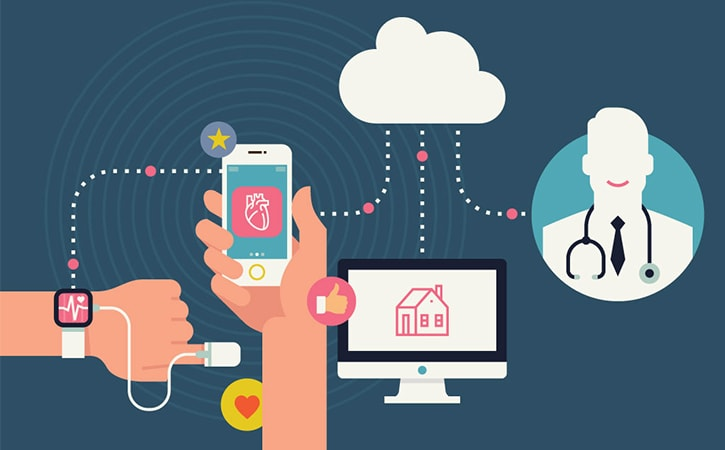
\includegraphics[width=0.7\linewidth]{img/benefits-of-iot-health-applications-of-iot.jpg}
            \caption{IoT Health}
            \label{fig:IoT-products-for-health}
        \end{figure}
        \item \textbf{Per la casa (Smart Home)}: il secondo scenario è rivolto alla domotica e all'uso di dispositivo per interagire con l'ambiente,
        come ad esempio l'apertura di una porta attraverso attuatori, controllo automatico della temperatura oppure il comando remoto delle luci tramite lo smartphone.
        \begin{figure}[h]
            \centering
            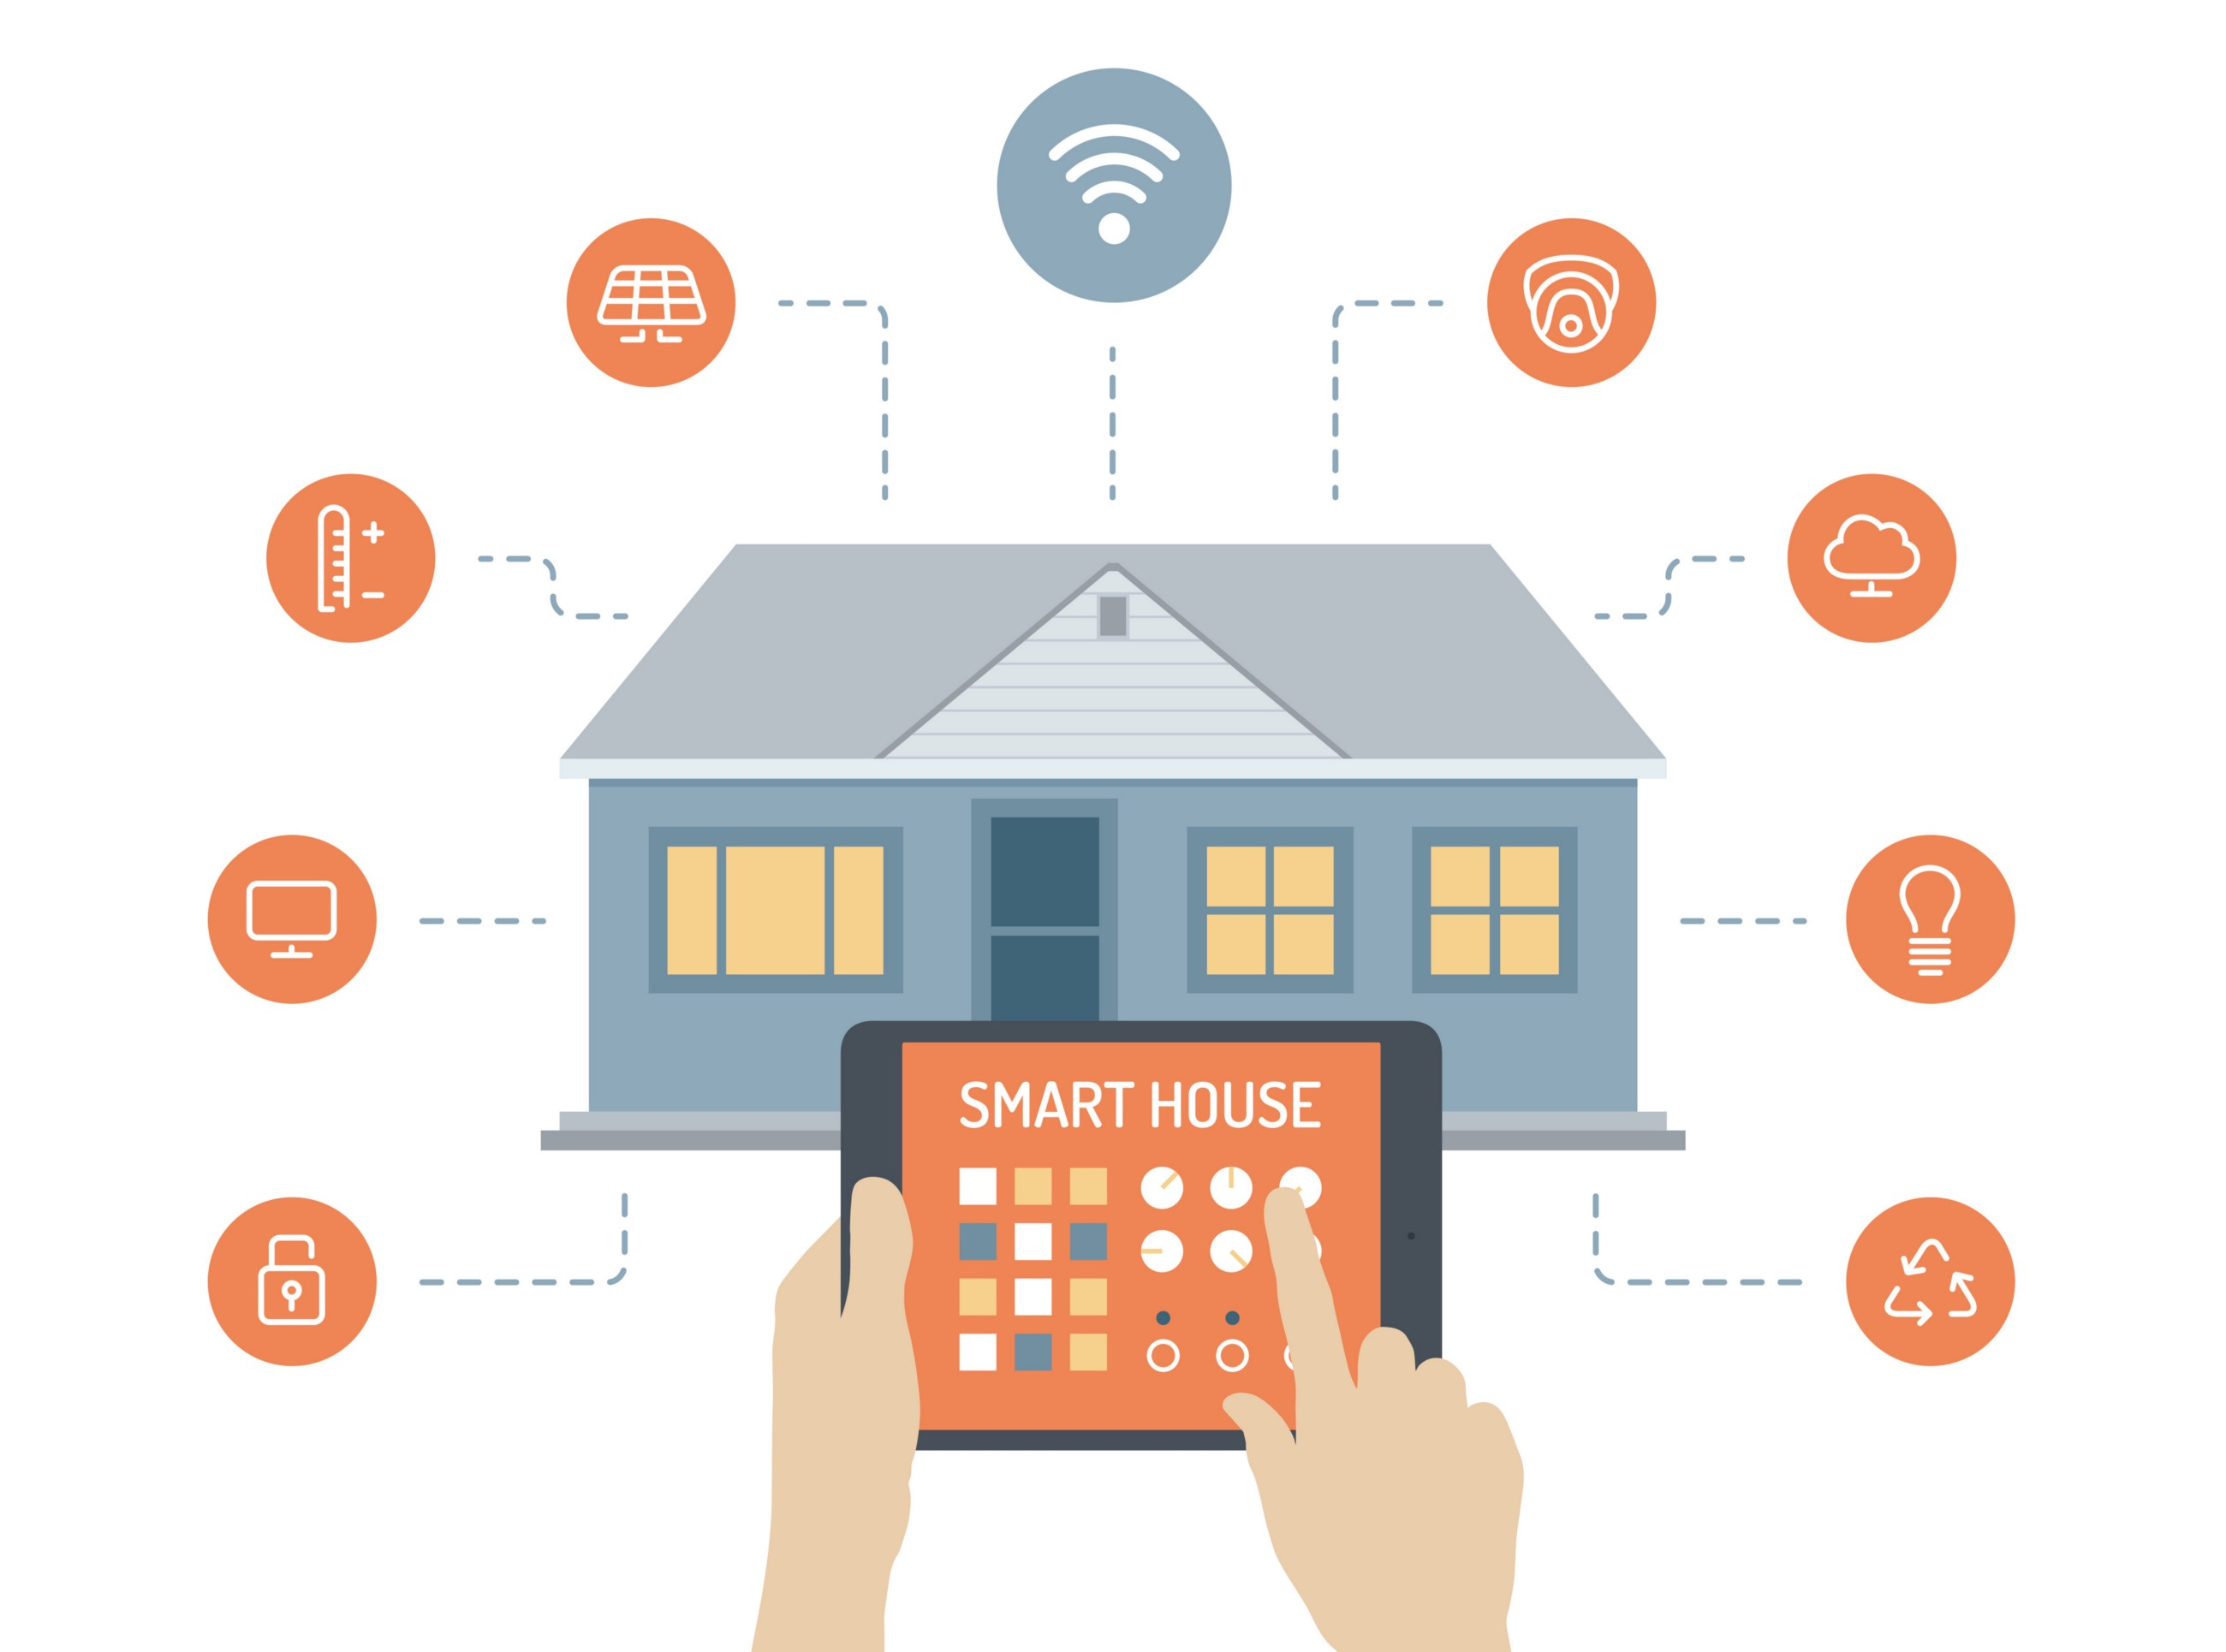
\includegraphics[width=0.7\linewidth]{img/smarthome.jpeg}
            \caption{IoT SmartHome}
            \label{fig:IoT-products-for-home}
        \end{figure}
        \item \textbf{Per la mobilità (Smart mobility)}: il terzo scenario prevede l'utilizzo dell'IoT per la creazione di smart mobility.
        L'individuazione di parcheggi liberi è un esempio di sistema IoT dove, attraverso sensori e/o telecamere ti aiutano a trovare parcheggio.
        Tutto questo, infatti, è basato su sensori che in tempo reale acquisiscono dati e trasmettono all'utente i dati richiesti. 
        \begin{figure}[h]
            \centering
            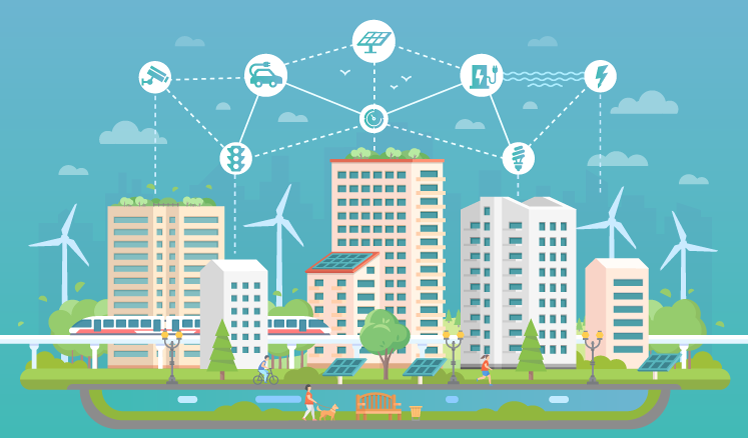
\includegraphics[width=0.6\linewidth]{img/smartcity.png}
            \caption{IoT smart mobility}
            \label{fig:-IoT-products-for-smart-mobility}
        \end{figure}
        \item \textbf{Per l'energia (Smart grid/ energy)}: il quarto scenario vede l'IoT in un contesto in cui si ha una gestione intelligente dell'energia.
        Questo sistema in maniera autonoma è in grado di indirizzare l'energia in tempo reale a dispositivi in cui in 
        quel momento serve più energia rispetto ad altri, o eventualmente cercare di equilibrare l'energia nel migliore dei modi.
        \begin{figure}[h]
            \centering
            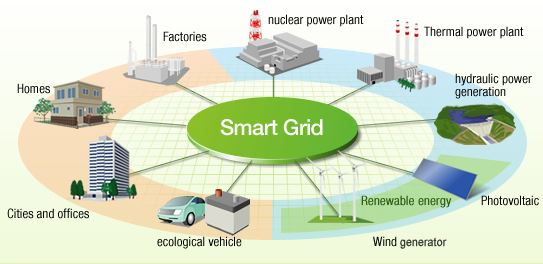
\includegraphics[width=0.6\linewidth]{img/smart_grid.jpg}
            \caption{IoT SmartGrid}
            \label{fig:IoT-products-for-smart-grid}
        \end{figure}
        \item \textbf{Per l'agricoltura}: il quinto scenario prevede l'utilizzo di sistemi IoT per l'agricoltura smart.
        Attraverso sensori di temperatura il sistema riesce a gestire il flusso d'acqua uscente per le piantagioni oppure riesce a capire quando accendere
        o spegnere l'erogazione di acqua.
        \begin{figure}[h]
            \centering
            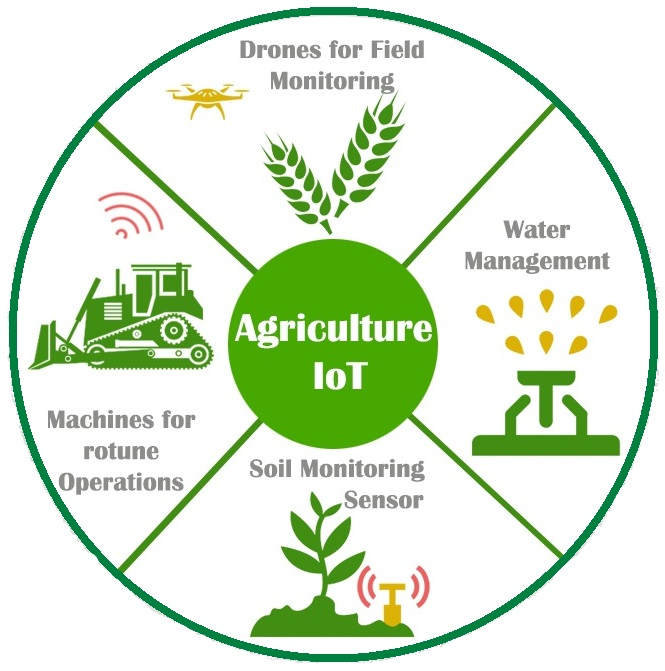
\includegraphics[width=0.5\linewidth]{img/agricolture.jpg}
            \caption{IoT Agricolture}
            \label{fig:IoT-products-for-agricolture}
        \end{figure}
        \pagebreak
        \item \textbf{Per le città smart (Smart Cities)}: il sesto scenario prevede l'applicazione di smart cities, ovvero un insieme di strategie di pianificazione
        urbanistica che mirano all'ottimizzazione e all'innovazione dei servizi pubblici così da mettere in relazione le infrastrutture materiali delle città.
        \begin{figure}[h]
            \centering
            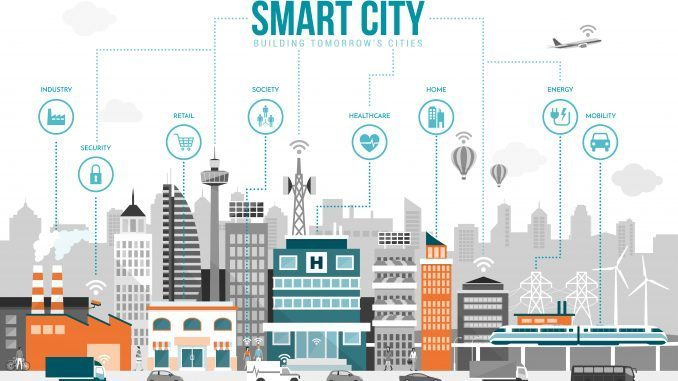
\includegraphics[width=0.5\linewidth]{img/smart-city.jpg}
            \caption{IoT Smart Cities}
            \label{fig:IoT-products-for-smartcities}
        \end{figure}
        \item \textbf{Industria 4.0}: l'ultimo scenario che vede lo sviluppo di sistemi IoT sono le industrie 4.0, denominate IIoT, nelle quali si cerca d'incrementare
        la produzione di oggetti e di migliorare la gestione e l'organizzazione dell'azienda stessa. L'industria 4.0 vuole rappresentare la quarta rivoluzione industriale.
        L'obiettivo principale nell'industria 4.0 è arrivare a una produzione massimamente diversificata, quindi rendere la produzione molto flessibile
        dal punto di vista produttivo. Il concetto di linea di produzione ben organizzata e inflessibile ora, con questo modello, viene abbandonata.
        Si inizia a parlare di Internet of Services, ovvero, la distinzione tra oggetti e servizi è talmente sottile che tutta l'infrastruttura viene vista e usata
        come un servizio.
        All'interno dell'industria anche le macchine devono adeguarsi ai sistemi IoT, infatti, le macchine devono avere le seguenti caratteristiche:
        \begin{itemize}
            \item {Inter-operabile}
            \item {Virtualizzabile}
            \item {Real-time}
            \item {Decentralizzata}
            \item {Orientata ai servizi e modulare}
        \end{itemize}
        Con queste caratteristiche una macchina è in grado di dialogare con il sistema e con l'ambiente in cui si trova cercando quindi di inviare
        informazioni sul proprio stato.
        Alla fine i dati devono essere interpretati, perché se a un dato non viene data la semantica non serve a nulla. 
        Una volta che i dati sono raccolti, vengono spediti nel cloud in cui verranno successivamente analizzati, rendendo possibile l'ottenimento di informazioni
        sullo stato dell'intero sistema e di conseguenza, se necessario, riuscire a modificare la produzione in tempo reale.
        \begin{figure}[h]
            \centering
            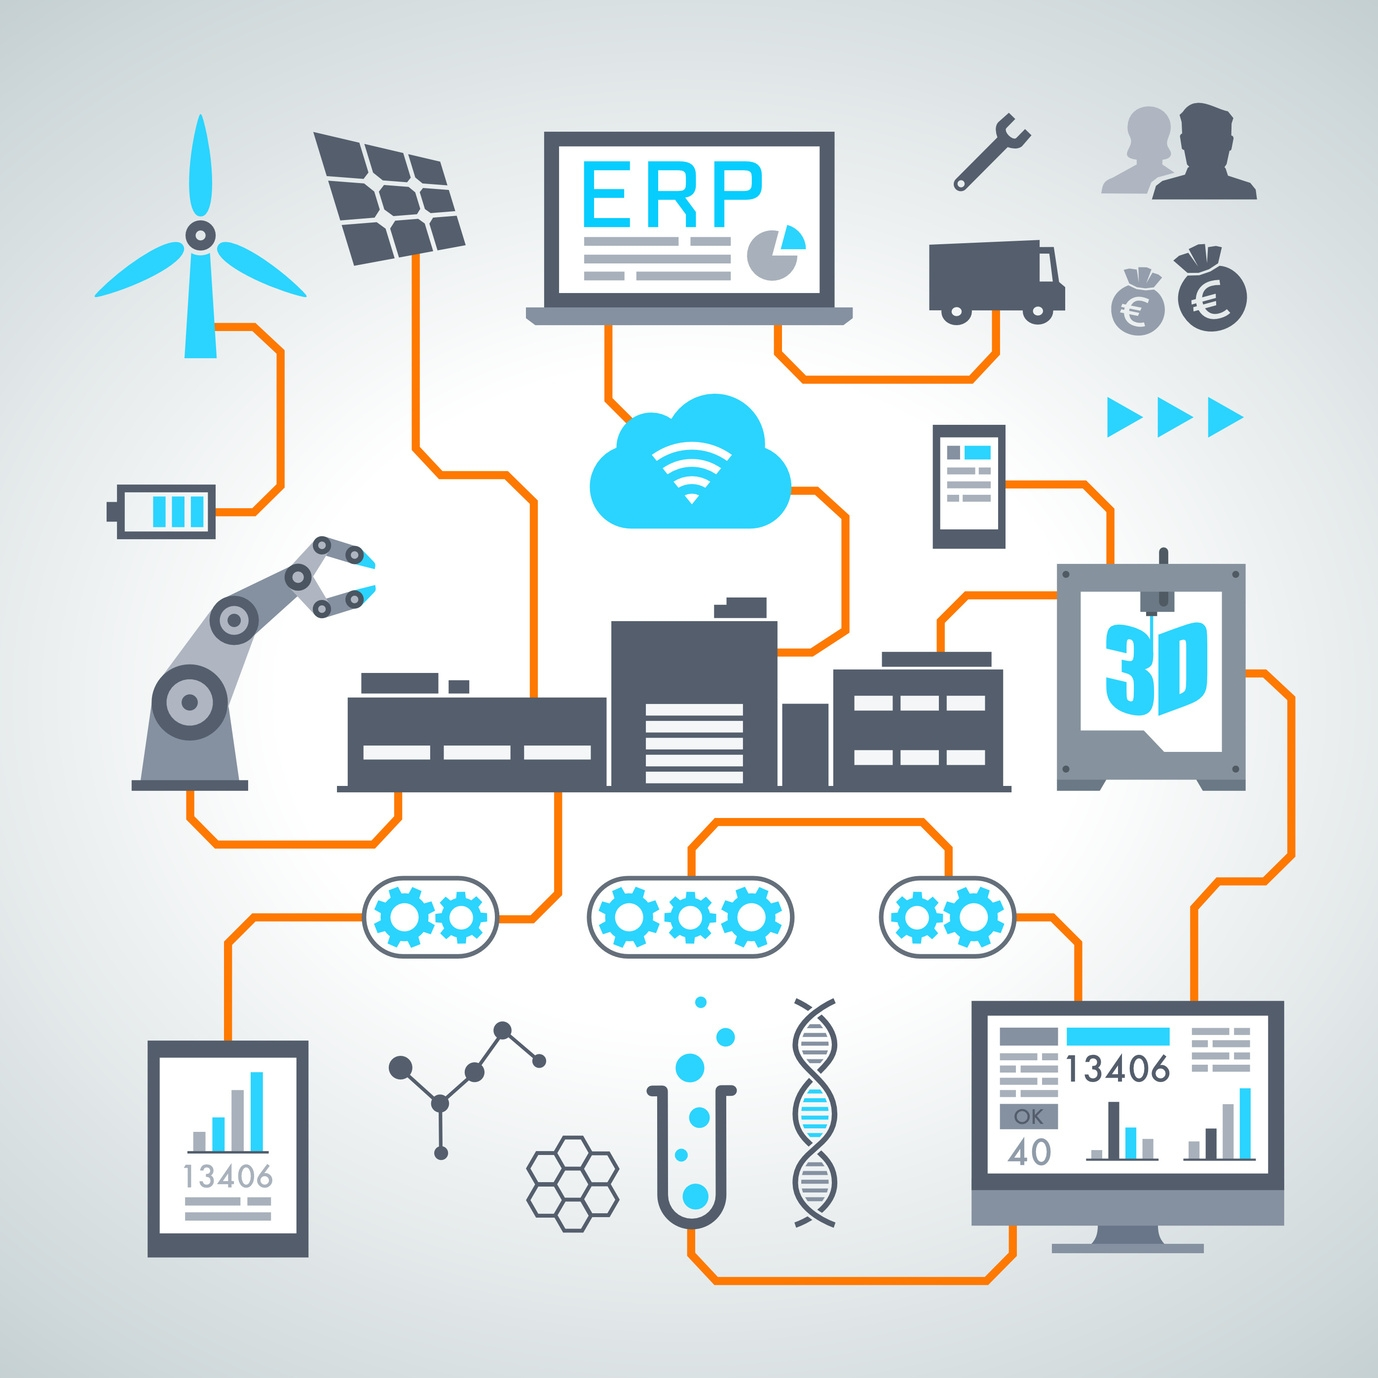
\includegraphics[width=0.5\linewidth]{img/industry.jpg}
            \caption{IoT Industry 4.0}
            \label{fig:IIoT}
        \end{figure}
    \end{itemize}
    \pagebreak
\subsection{Ingredienti per una soluzione IoT}
La realizzazione di IoT è composta da alcuni layers:
\begin{itemize}
    \item \textbf{Device layer}
    \begin{itemize}
        \item Sensori
        \item Attuatori
        \item Tagged devices/objects
    \end{itemize}
    \item \textbf{Communication layer}
    \begin{itemize}
        \item Device gateway
        \item Smart gateway
        \item Protocollo di comunicazione
        \item Protocollo applicativo
        \item Protocollo industriale
    \end{itemize}
    \item \textbf{Core platform}
    \begin{itemize}
        \item Protocol Gateway
        \item IoT Messagging Middleware
        \item Data storage
        \item Data aggregation/filter
    \end{itemize}
    \item \textbf{Analytics platform}
    \begin{itemize}
        \item Processo di streaming
        \item Machine Learning
        \item Eventi e report
    \end{itemize}
\end{itemize}
È importante ricordare che, oltre, all'architettura, alla raccolta e gestione dei dati è importante avere un buon livello di
sicurezza per l'invio e la gestione dei dati sensibili. 

Nel \textbf{device layer} ci sono i dispositivi in sè, che permettono di acquisire dati e inviarli tramite internet.
Di solito questi dispositivi embedded dotati di un micro-controllore, una memoria, eventuali interfacce e un sistema operativo dedicato
in base al contesto in cui sono piazzati. Il più delle volte sono dotati di architetture low power per poter risparmiare energia,
in quanto alimentati da batteria. Qualsiasi dispositivo IoT è dotato di sensori, senza i quali non sarebbe possibile la raccolta dati.

I sensori possono essere di qualsiasi tipologia: elettronici, meccanici, idraulici, ecc. Ciò che li contraddistingue è il fatto di
essere ``smart'', ovvero dotati già a livello sensoriale di componenti logiche che eseguono un minimo di data-processing.
\begin{figure}[h]
    \centering
    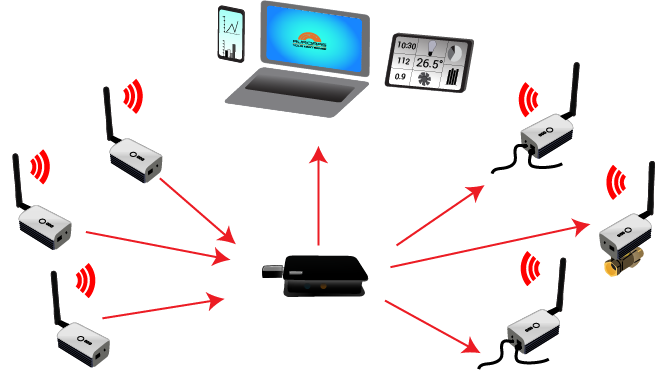
\includegraphics[width=0.5\linewidth]{img/sensori.png}
    \caption{IoT sensors}
    \label{fig:Sensors}
\end{figure}\\
Gli \textbf{attuatori} sono dispositivi che permettono d'interagire con l'ambiente in cui si trovano, in base a un'azione inviata come input.
\begin{figure}[h]
    \centering
    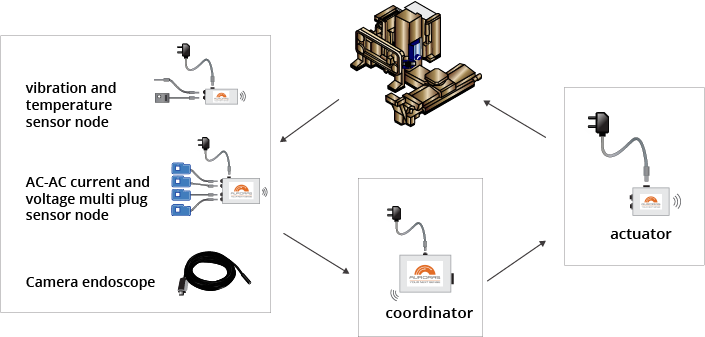
\includegraphics[width=0.6\linewidth]{img/TELEMETRY3.png}
    \caption{IoT actuators}
    \label{fig:Actuators}
\end{figure}

Esistono anche dispositivi non alimentati che permettono però di poter interagire attivamente con l'ambiente. Spesso questo avviene tramite meccanismi
come l'RFID (Radio Frequency Identification), che tramite circuiti integrati alimentati durante l'utilizzo inviano i dati contenuti al lettore, che poi
si occuperà dell'eventuale invio dei dati su internet.
\begin{figure}[h]
    \centering
    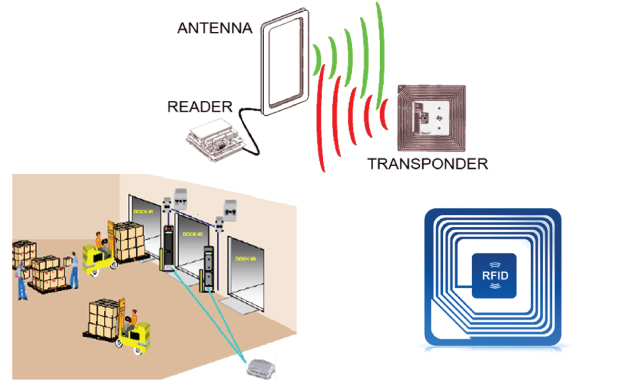
\includegraphics[width=0.6\linewidth]{img/rfid.jpg}
    \caption{IoT RFID}
    \label{fig:RFID}
\end{figure}

Per avere invece una comunicazione \textbf{bidirezionale} si usa l'NFC (Near Field Communication), che lavorando con frequenze molto corte costringe 
l'interazione ad avvenire in maniera ravvicinata.
\begin{figure}[h]
    \centering
    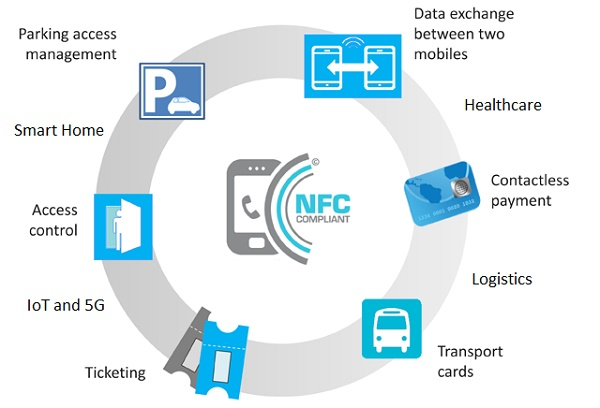
\includegraphics[width=0.6\linewidth]{img/NFC-applicatioins.jpg}
    \caption{IoT NFC}
    \label{fig:NFC}
\end{figure}
\pagebreak

Altra tecnologia molto diffusa sono i \textbf{beacons}, un'ulteriore forma di tagged devices, che sfrutta la tecnologia \textbf{bluetooth LE (Low Energy)}
per trasmettere un segnale in broadcast per indicare, di solito, la posizione ad altri ricevitori bluetooth. La trasmissione bluetooth si può usare in diversi contesti.
\begin{figure}[h]
    \centering
    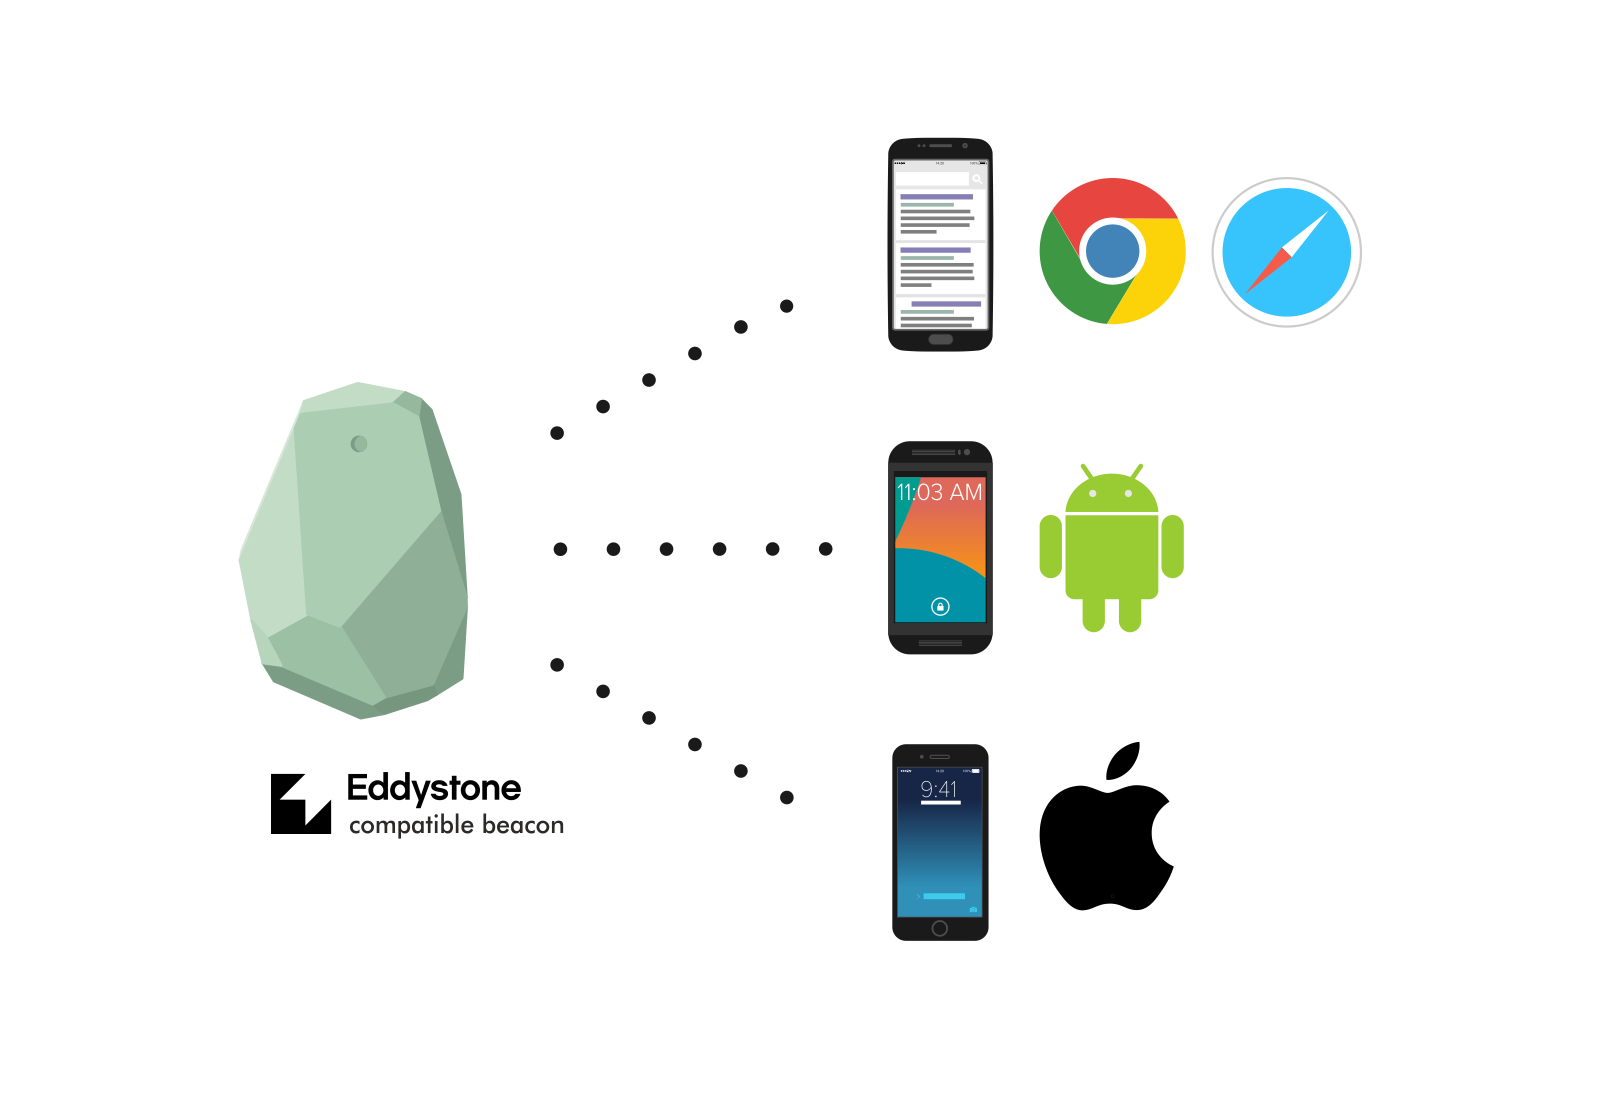
\includegraphics[width=0.6\linewidth]{img/eddystone.png}
    \caption{IoT Beacon}
    \label{fig:Beacon}
\end{figure}

Il \textbf{communication layer} indica la parte di comunicazione dal dispositivo locale verso la rete internet.
Qui si possono distinguere dispositivi che sono in grado di connettersi alla rete, attraverso Wi-Fi o rete cellulare (3G/4G) e dispositivi che non sono 
in grado di connettersi direttamente a internet e quindi per poterlo fare hanno bisogno di connettersi a un \textbf{gateway o un hub}, con il quale è possibile 
arrivare alla rete esterna. Spesso il gateway sono anch'essi ``smart'': esso ha una propria memoria interna e delle specifiche appliccazioni embedded che 
permettono di analizzare i dati direttamente sul posto prima di instradarli verso un altro gateway o un hub centrale.

Più specificamente, gli smart gateway permettono:
\begin{itemize}
    \item \textbf{Filtraggio e aggregazione di dati}: cercano di dare una semantica ai dati ricevuti e scartare quelli inutili.
    \item \textbf{Buffering}: quando un dispositivo rimane offline, hanno un certo buffer per mantenere in memoria i dati trasmessi
    \item \textbf{Sincronizzazione}: aggiornamento dei dati mancanti o incompleti
\end{itemize}
Un'applicazione sul campo di questi smart gateway può essere la smart city. Per esempio, un lampione può fare da smart gateway e comunicare i dati da una zona a un'altra.
Gli stessi smartphone possono essere considerati dei gateway, infatti nel momento in cui comunicano con una smartband oppure uno smartwatch,
sono loro che ricevono i dati e li inviano alla rete.

I \textbf{protocolli di comunicazione} sono responsabili per la connettività di rete.
Alcuni protocolli più usati per una connessione diretta verso internet sono:
\begin{itemize}
    \item Wi-Fi
    \item Ethernet
    \item Rete cellulare (3G,4G, in futuro 5G)
\end{itemize}
Non tutti i protocolli sono in grado di connettere i dispositivi direttamente a internet, ad esempio:
\begin{itemize}
    \item Bluetooth (LE)
    \item RFID
    \item NFC
    \item Zigbee/Z-wave
\end{itemize}
I \textbf{protocolli di applicazione} poggiano, come nei normali PC general purpose, sul protocollo TCP/IP.
Nel caso dei dispositivi IoT viene data molta enfasi all'uso del cloud, motivo per cui si sono creati protocolli specifici.
In particolare, i due procotolli più usati e più "famosi" sono \textbf{MQTT} e \textbf{AMQP}.
\textbf{MQTT} è stato pensato per trasferire dei dati che partono da un database locale, per esempio all'interno di un'azienda.
\textbf{AMQP} a differenza di MQTT garantisce una minore latenza nel trasferimento dei dati, questo perchè l'uso del protocollo AMQP 
è stato pensato per applicazioni IoT, infatti i dati che vengono trasferiti sono di piccole dimensioni e la trasmissione può essere asincrona.

Alla base del protocollo \textbf{MQTT} (Message Queue Telemetry Transport) si trova il classico concetto di \textbf{publisher e subscriber}.
Viene ssato principalmente per:
\begin{itemize}
    \item Invio di dati con una taglia molto piccola
    \item Dispositivi dotati di hardware limitato
    \item Rete con poca banda e alta latenza
\end{itemize}
Il payload dei messaggi essendo binario risulta molto compatto. Come detto prima, questo protocollo sfrutta il concetto di \textbf{publisher e subscriber}.
Tutti i dispositivi IoT che sono presenti nella rete si connettono a un \textbf{broker MQTT}.
Il broken MQTT sopporta molteplici connessioni con un numero elevato di dispositivo connessi ad esso.
Una volta che un client vuole connettersi al broken, invia un messaggio di "benvenuto" e si sottoscrive ad uno o più \textbf{topic}.
Un topic è una stringa con formato UTF-8 che viene usata dal broken per filtrare i messaggi da inviare ai client sottoscritti a diversi topic. I topic possono essere composti da un solo livello o a più livelli.
Un client può decidere di sottoscriversi ad uno o più topic usando una \textbf{wildcards}.
Per identificare se un client è sottoscritto ad uno o più topic nella wildcard c'è un carattere speciale che identifica, single-level con la `$+$' o multi-level con `$\#$'.
Il protocollo MQTT permette anche la \textbf{QoS}, ovvero, la Quality of Services che garantisce, con un livello di accuratezza, la garanzia che quel messsaggio venga inviato al destinatario.\\
Per la QoS ci sono 3 livelli:
\begin{itemize}
    \item 0: Al massimo una volta
    \item 1: Almeno una volta
    \item 2: Esattamente una volta
\end{itemize}
Se vogliamo possiamo pensare all'invio del messaggio come ad un ack a livello TCP/IP, perchè anche qui ci sono sempre due parti di invio e ricezione del messaggio.
\begin{itemize}
    \item I messaggi che partono dal client e arrivo al broken: in questo caso il livello di QoS dipende dal livello che il client ha settato nel messaggio in cui ha appena inviato.
    \item I messaggi dal broken verso il client: in questo caso il livello di QoS usato dal broken \textbf{non} è quello usato nel messaggio appena inviato dal client, ma, il livello di QoS che il client aveva settato in precendeza.
\end{itemize}
Il broken ha alcune funzionalità di store, il quale, salva l'ulitmo messaggio inviato in quel topic.\\
Ogni volta che un client si collega al broken, oltre, al messaggio di benvenuto che si scambiano all'inizio, inviano anche il testamento di fine connessione, nel quale, viene definito ciò che deve fare il broken una volta che questo si disconnette dalla rete. Il broken, infatti, tiene in memoria il testamento finchè il client non esce dalla rete.
\begin{figure}[h]
    \centering
    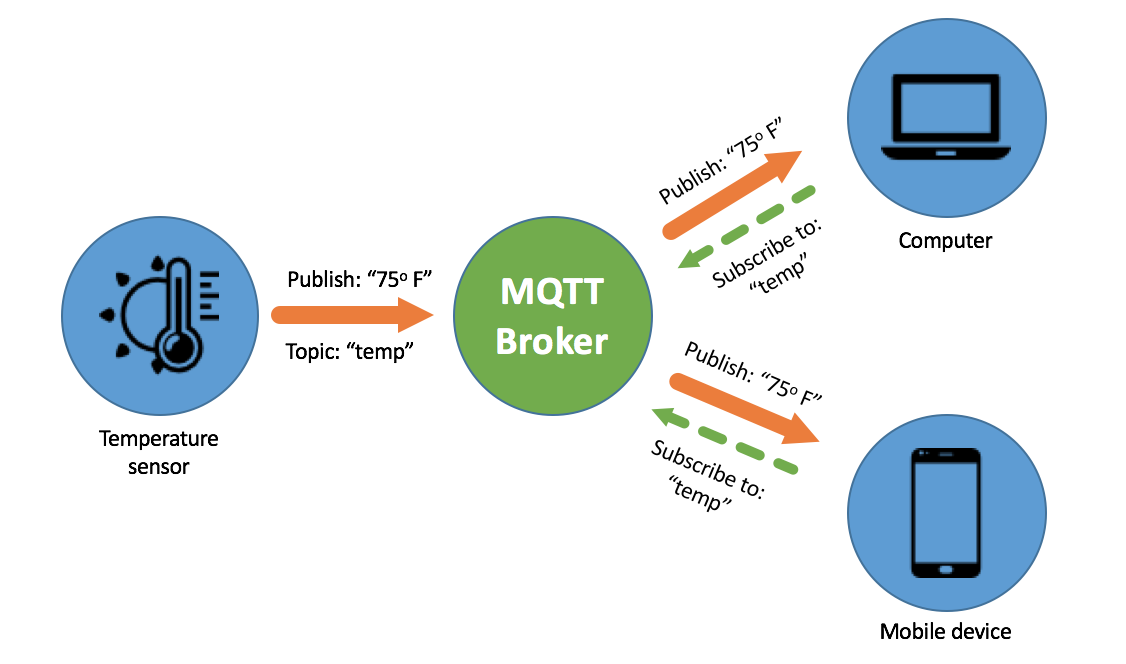
\includegraphics[width=0.6\linewidth]{img/MQTT.png}
    \caption{MQTT}
    \label{fig:MQTT}
\end{figure}


Il protocollo \textbf{AMQP} (Advanced Message Queuing Protocol), è molto simile al protocollo MQTT. Anche questo protocollo è basato su TCP/IP. Il protocollo AMQP supporta sia il modello basato su coda che quello publisher e subscriber.

I \textbf{protocolli industriali} sono soluzioni che vengono adottate soprattutto in ambito industriale.
Ci sono due protocolli molto famosi:
\begin{itemize}
    \item \textbf{SCADA}
    \item \textbf{ModBus}
\end{itemize}
In particolare, il protocollo ModBus mi permette di dialogare con le macchine e di estrapolare i dati in maniera da poter attribuirgli un significato. Infatti, assieme a ModBus viene spesso utilizzato \textbf{OPC-UA} che è uno standard in cui i dati devono assumere una certa struttura per poter essere interpretati dalle applicazioni in futuro applicate. Quindi OPC-UA mi permette di definire una certa \textbf{semantica} ai dati che la macchina produce. 
Il \textbf{Core Platform} lo possiamo vedere come una sorta di grande hub o gateway in grado di dialogare con più protocoll diversi tra loro e di connettere moltissimi dispositivi assieme.
Il core platform è composto da:
\begin{itemize}
    \item \textbf{Protocol Gateway}
    \item \textbf{IoT Messagging Middleware}
    \item \textbf{Data storage}
    \item  \textbf{Data aggregation / filter}
\end{itemize}
Il \textbf{Protocol Gateway} è la parte principale del Core Platform perchè è in grado di garantire la trasparenza di più protocolli diversi tra loro, gestendo la tua soluzione IoT.

L'\textbf{IoT Messagging Middleware} è un software presente nel Core Platform molto simili ai protocolli visti in precedenza, MQTT e AMQP perchè adotta il modello publisher e subscriber.
Prima abbiamo definito il Core Platform come un grande hub che è in grado di gestire moltissimi dispositivi connessi ad esso, tutto questo, infatti, è derivante dall'IoT Messagging Middleware che permette di avere elevate performance e tolleranza al guasto.\\
Questo livello permette, inoltre, di lavorare con meta-modelli.\\
Questi meta-modelli vengono definiti attraverso l'emissione di dati dai diversi dispositivi. I meta-modelli permettono di creare una soluzione dipendente dai dati inviati dai dispositivi e quelli che vengono usati piattaforma IoT. Tramite queste astrazioni il software è in grado di gestire più tipi di dati dai diversi protocolli. Infine, l'IoT Messagging Middleware permette uno storage di particolati intervalli di dati cercando di analizzare i dati che gli stanno arrivando. Poi capiamo meglio come i dati vegono analizzati nei livelli successivi.

Nel livello \textbf{Data Storage} come dice il termine stesso è il livello che si occupa di immagazzinare i dati in Database per poter avere una copia locale.
I Database più utilizzati sono:
\begin{itemize}
    \item \textbf{MongoDB}
    \item \textbf{CouchDB}
\end{itemize}
Nel livello \textbf{Data Aggregation and filter} i dati vengono convertiti in alcuni formati specifici per poter poi essere mandati ad un software in grado di creare dei modelli di dati per essere interpretati.\pagebreak
\\
L'ultimo livello, per una soluzione IoT, è l'\textbf{Analytics Platform Layer} il quale permette di analizzare una grande mole di dati, di predirre un dato e di eseguire una determinata azione.
Quest'ultimo livello è composto da:
\begin{itemize}
    \item \textbf{Stream processing}
    \item \textbf{Machine Learning}
    \item \textbf{Actionable Insights}
\end{itemize}
Nello \textbf{Stream processing} vengono ricevuti i dati in tempo reale dai dispositivi e analizzati in maniera da trovare delle correlazioni tra i differenti dati per poter poi successivamente usare quest'informazione per migliorare qualcosa.

Per \textbf{Machine Learning} si intende l'apprendere delle nozioni sui dati che abbiamo senza esplicitamente creare degli algoritmi per farlo. CI sono 4 fasi principali per utilizzare questo meccanismo:
\begin{itemize}
    \item Capire il problema e trovare una soluzione
    \item Pulire i dati e analizzare i dati filtrati
    \item Creare dei modelli (es. IoT Messagging Middleware)
    \item Fare training sui dati
\end{itemize}
Detto questo, però, ci sono 3 modi per eseguire Machine Learning:
\begin{itemize}
    \item \textbf{Supervised learning}: I dati che arrivano dall'esterno sono già etichettati, pronti per essere interpretati e riuscire a predirre i dati successivi.
    \item \textbf{Unsupervised learning}: I dati che arrivano dall'esterno non sono già stati manipolati e qui è l'algoritmo stesso che capisce dove sono le correlazioni tra i dati. 
    \item \textbf{Reinforcement learning}: Il sistema impara dai dati che riceve dall'ambiente esterno, per esempio, attrverso un sensore.
\end{itemize}
Il livello \textbf{Actionable Insights} permette di creare report degli eventi in base ai dati che vengon analizzati.

\subsection{Cloud}
Anche se non è parte integrante di una soluzione IoT il \textbf{Cloud} è la parte fondamentale per rendere il sistema IoT.\\
Per Cloud si intende un'area in cui i dati da diversi dispositivi vengono inviati attraverso internet.\\
Il Cloud può essere di due tipi:
\begin{itemize}
    \item \textbf{Privato}: La gestione e il mantenimento del cloud è a carico di chi ha creato il cloud, senza potersi appoggiare ad altri enti. Molte aziende utilizzano questa tipologia di cloud per paura di condiviedere i dati ad altri enti. 
    \item \textbf{Pubblico}: La gestione e il mantenimento del cloud è a carico di chi gestisce il servizio di cloud. Chi usufruisce del servizio paga lo spazio che utilizza.
\end{itemize}
\begin{figure}[h]
    \centering
    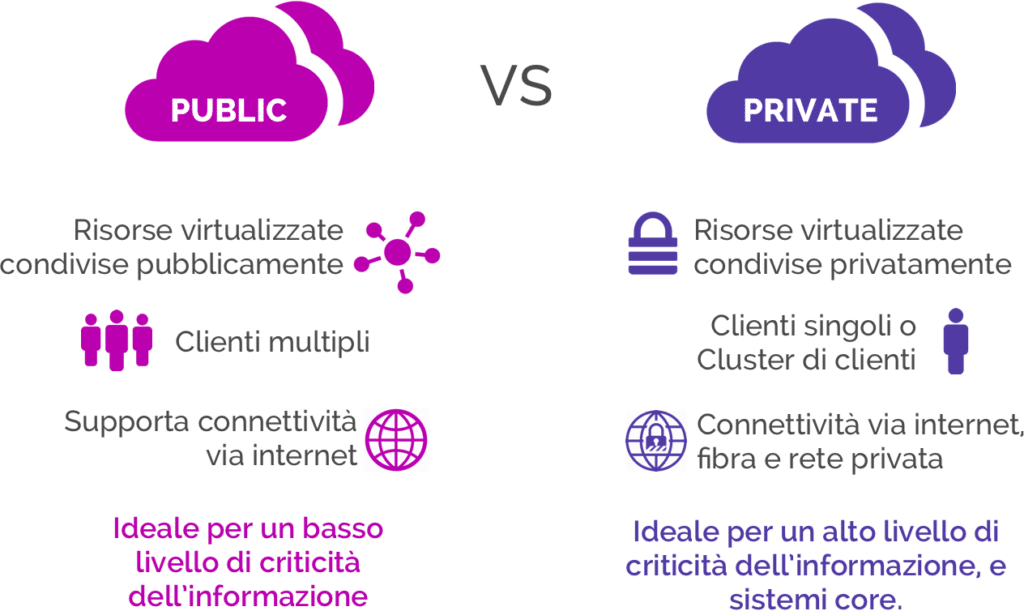
\includegraphics[width=0.6\linewidth]{img/Cloud.png}
    \caption{Cloud}
    \label{fig:Cloud}
\end{figure}
La soluzione migliore è quella di creare un \textbf{Cloud Ibrido}, ovvero, che ha sia la parte di computazione privata, esempio dati sensibili di un'azienda, e la computazione dei dati ormai filtrati all'esterno, senza conpromettere la "privacy" dei dati.\\
Nel momento in cui la scelta ricade su un cloud pubblico ci possono essere delle categorie di servizi offerti come: \textbf{IAAS – PAAS - SAAS}

\textbf{IASS (Infrastructure as a Service)}: Questo tipo di servizio include offerte come lo spazio virtuale su server, connessioni di rete, larghezza di banda, indirizzi IP e bilanciatori di carico. Fisicamente, il gruppo di risorse hardware viene estratto da una moltitudine di server e reti solitamente distribuiti presso numerosi Data Centre, la cui manutenzione è responsabilità del provider del cloud.

\textbf{PAAS (Platform as a Service)}: Consente agli utenti di creare applicazioni software utilizzando gli strumenti forniti dal provider.\\
Le funzioni che possono essere incluse in un'offerta PaaS sono:
\begin{itemize}
    \item Sistema operativo
    \item Ambiente di programmazione lato server
    \item Sistema di gestione database
    \item Software server
    \item Assistenza
    \item Archiviazione
    \item Accesso di rete
    \item Strumenti per progettazione e sviluppo 
    \item Hosting
\end{itemize}
\textbf{SAAS (Software as a service)}: Indica qualsiasi servizio cloud tramite il quale i consumatori possono accedere ad applicazioni software tramite internet.\\
Spesso viene chiamato "software on demand", in quanto il suo utilizzo è più simile a un noleggio del software che al suo acquisto.
\begin{figure}[h]
    \centering
    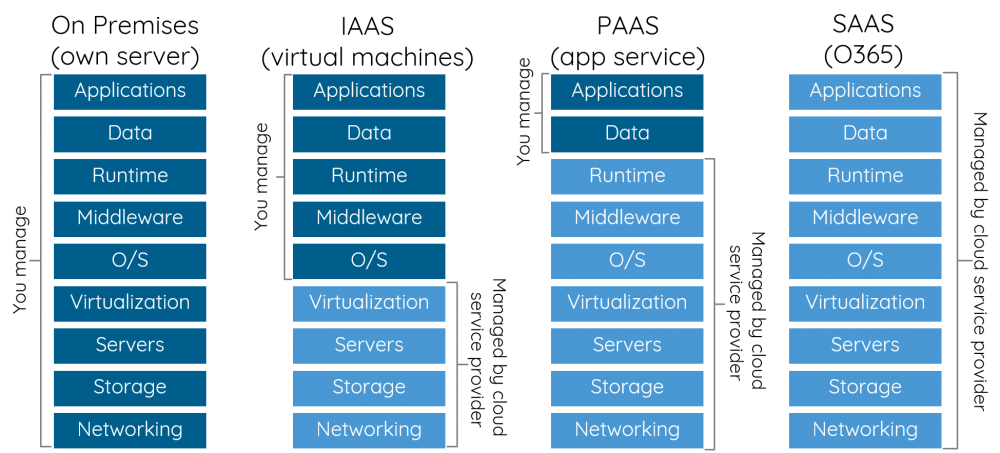
\includegraphics[width=1\linewidth]{img/Cloud-service.png}
    \caption{Cloud Services models}
    \label{fig:Cloud Services models}
\end{figure}
\subsection{Architettura cloud per IoT}
Alla fine, come detto all'inizio, una soluzione IoT oltre a tutti gli ingredienti visti fin'ora ha bisogno della rete internet per poter comunicare con il mondo esterno, ma soprattutto, dei cloud per poter racogliere in un'unico spazio i dati raccolti e poterli esaminare e ottenere dei risultati validi.

\begin{figure}[h]
    \centering
    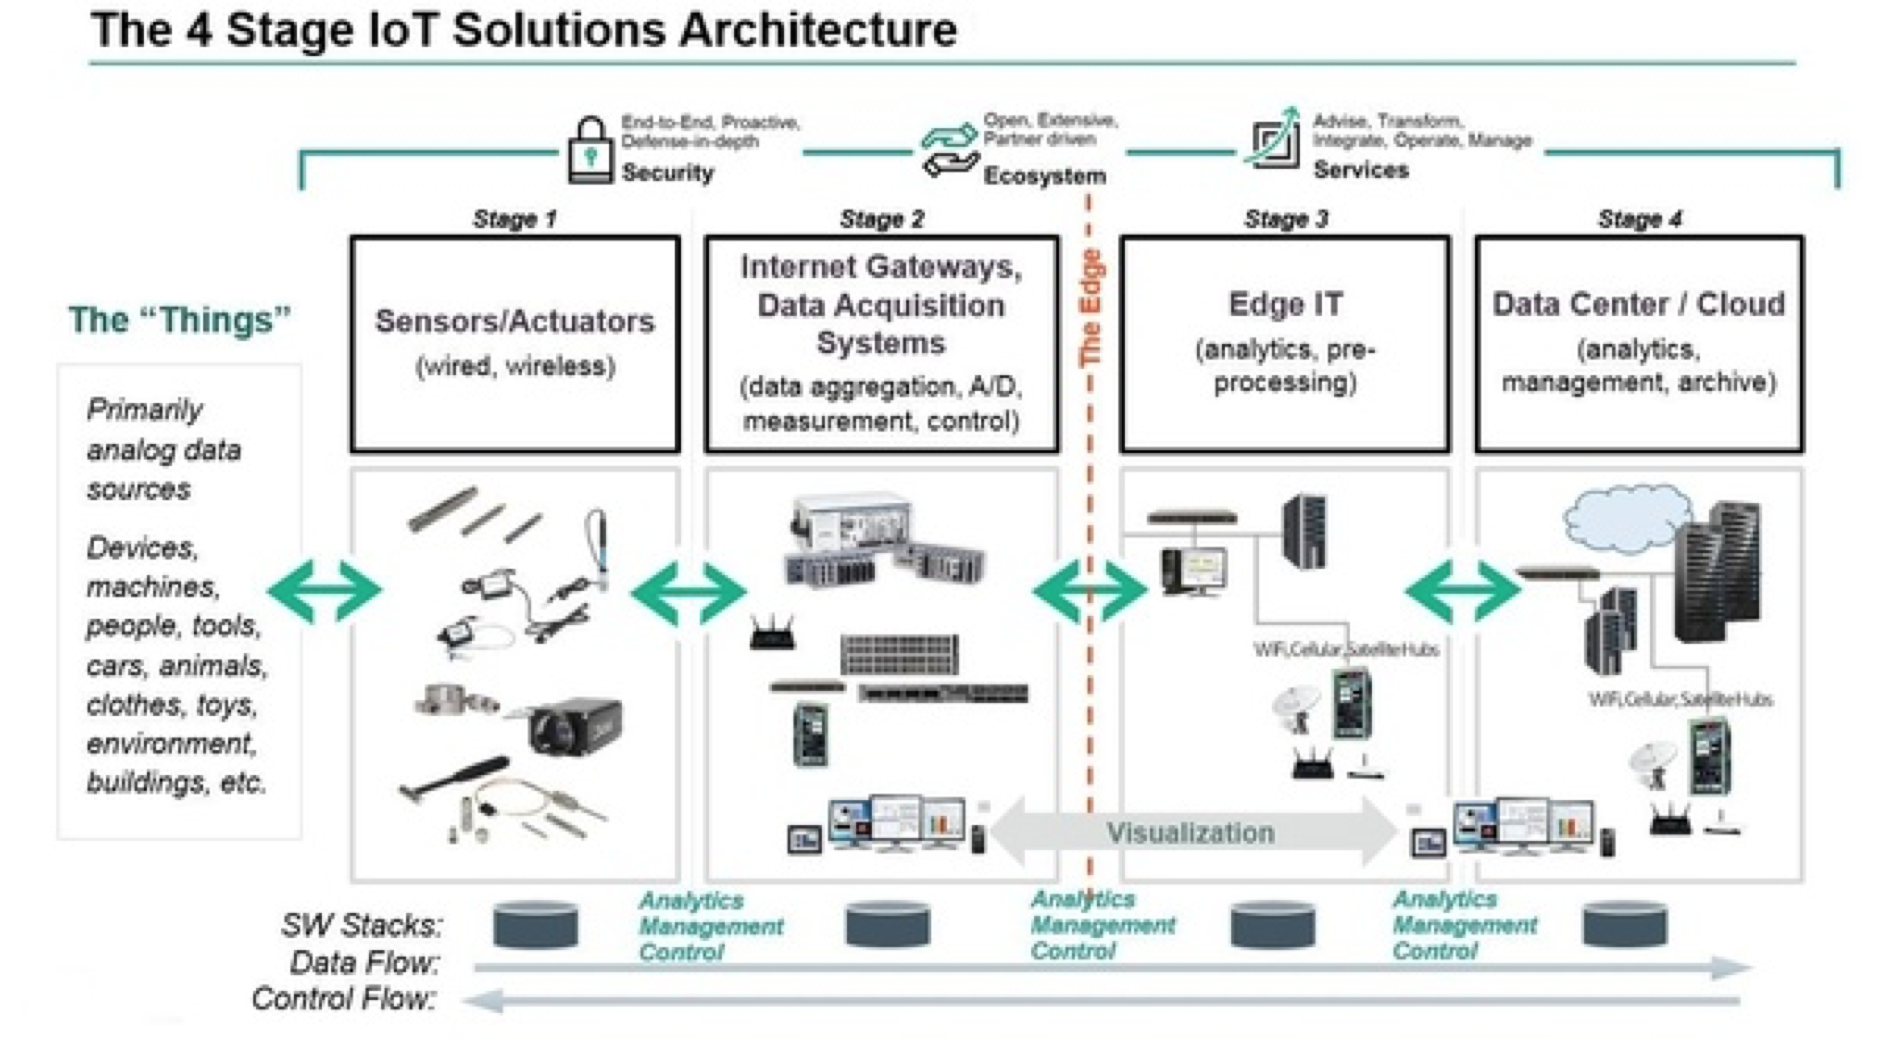
\includegraphics[width=1\linewidth]{img/arch_iot.png}
    \caption{Cloud Architecture for IoT Solution}
    \label{fig:Cloud Architecture for IoT Solution}
\end{figure}
\end{document}

